\documentclass[draft]{agujournal2019}
\usepackage{url}
%\usepackage{hyperref}
\usepackage{lineno}
\usepackage{todonotes}
\usepackage{subcaption}
\usepackage[inline]{trackchanges} %for better track changes. finalnew option will compile document with changes incorporated.
\usepackage{soul}
\linenumbers
%%%%%%%
% As of 2018 we recommend use of the TrackChanges package to mark revisions.
% The trackchanges package adds five new LaTeX commands:
%
%  \note[editor]{The note}
%  \annote[editor]{Text to annotate}{The note}
%  \add[editor]{Text to add}
%  \remove[editor]{Text to remove}
%  \change[editor]{Text to remove}{Text to add}
%
% complete documentation is here: http://trackchanges.sourceforge.net/
%%%%%%%

\draftfalse
%\setlength {\marginparwidth }{2cm}

\journalname{JGR: Space Physics}

\begin{document}

\title{Coordinate Systems and Transforms in Space Physics: Terms, Definitions, Implementations, and Recommendations for Reproducibility}

\authors{R.S. Weigel, A.Y. Shih, R. Ringuette, I. Christopher, S.M. Petrinec, S. Turner, R.M. Candey, G.K. Stephens, B. Thomas, and B. Cecconi}

%\todo[inline]{Turner, Thomas, Christopher, Cecconi -- verify that no middle initial used in papers.}

%\todo[inline]{Petrinec and Turner -- verify that you don't have ORCID}

%\todo[inline]{All others -- verify ORCID below}

%\todo[inline]{(Bobby): Would we want to ask Russell or Hapgood or others to review?}

%https://archive.org/details/referenceframesi0000unse/page/47/mode/1up?view=theater

% Send Steve Joy draft


\noindent
%Weigel https://orcid.org/0000-0002-9521-5228\\
%Shih https://orcid.org/0000-0001-6874-2594\\
%Ringuette https://orcid.org/0000-0003-0875-2023\\
%Cecconi https://orcid.org/0000-0001-7915-5571\\
%Candey https://orcid.org/0000-0002-4698-8769\\
%Thomas https://orcid.org/0000-0003-1623-9035\\
%Christopher https://orcid.org/0000-0002-0262-6432\\
%Stephens https://orcid.org/0000-0002-5961-5582\\
%\vspace{0.2in}

%\affiliation{1}{George Mason University, 4400 University Drive, Fairfax, VA 22030}
\correspondingauthor{R.S. Weigel}{rweigel@gmu.edu}

%  List up to three key points (at least one is required)
%  Key Points summarize the main points and conclusions of the article
%  Each must be 140 characters or fewer with no special characters or punctuation and must be complete sentences


\begin{keypoints}
\item Reproducing coordinate system transforms is difficult due to variations in definitions and implementations in the software typically used.
\item Ephemeris from different providers can differ significantly (${\sim}0.3^\circ$), as do Z--axis orientations from surveyed software libraries (${\sim}0.03^\circ$).
%\item The resulting precision of (${\sim}0.3^\circ$) in ephemeris and (${\sim}0.03^\circ$) in Z–axis orientations has now become problematic for spacecraft constellation operations.
\item We present recommendations to improve the precision and reproducibility of these calculations and reduce expensive duplication by missions.
\end{keypoints}

%\item Reproducing coordinate system transforms is difficult due to variations in definitions and implementations; recommendations are given to address.
%\item Ephemeris from different providers can differ significantly (${\sim}0.3^\circ$), as do Z--axis orientations from surveyed software libraries (${\sim}0.03^\circ$).
%\item There is duplication of effort by spacecraft missions related to coordinate system transform calculations.
%\item Recommendations are given to make reproducibility easier and reduce duplication of effort.

% Albert - we will add although the focus is on space physics, similar issues and recommendations apply to solar. Can you give a few examples?

\begin{abstract}
In space physics, acronyms for coordinate systems (e.g., \texttt{GEI}, \texttt{GSM}) are commonly used; however, differences can exist in their definitions and implementations that prevent reproducibility. In this work, we compare definitions in frequently cited journal articles, online resources, and software packages and show that implementation differences can lead to transformations between same--named coordinate systems to differ significantly. Based on these comparisons and results, and to enable reproducibility, we recommend that (a) a standard for acronyms and definitions for coordinate systems is developed; (b) a central authority maintains a citable database of reference data needed for these transforms;  (c) a central authority maintains the SPICE (Spacecraft, Planet, Instrument, C-matrix, Events) kernels used by transforms by space physics spacecraft missions to generate data products in different coordinate systems; and (d) software developers provide explicit comparisons of their implementations with the results of (b) and documentation on implementation choices. In addition, we provide recommendations for scientists and metadata developers to ensure that sufficient reproducibility--enabling information is provided in the absence of these recommendations being implemented.
\end{abstract}

\section{Introduction}

In space physics journal articles and software, the definition of a coordinate system is typically given by citing a reference that describes it. (Thus far, we have used the term ``coordinate system" consistent with common usage in space physics. In section~\ref{sect:terminology}, we note that ``ideal reference system", ``reference system", or ``reference frame" is more consistent with literature outside of space physics and will use these terms in the remainder of this article.)
This work stems from a project to develop a standard for ideal reference system acronyms such as \texttt{GEI}, \texttt{GSE}, \texttt{GSM}, and their commonly used variations, e.g., \texttt{GEI\_J2000}, \texttt{GEI\_MOD}; see the section~\ref{sect:glossary} for definitions. The motivation was that, given a statement such as ``the vector measurements in \texttt{ABC} were transformed into \texttt{XYZ}," a scientist with measurements in \texttt{ABC} would be able to reproduce the transformation with the only uncertainty being due to round--off error at the level of floating point precision.

The primary challenge with this task is that implementing a given reference system requires making implementation choices, and therefore, definitions of reference implementations are also needed (in section~\ref{sect:definitions}, we refer to an implementation of a reference system as a ``reference frame"). As a result, developing a list of acronyms and associated definitions for reference systems does not address the fundamental problem of reproducibility --- implementations of the same reference system will not necessarily be the same because implementations rely on models, and there are both independent models and multiple versions of the same model that can be used.

In section~\ref{sect:comparisons_ephemeris}, we give an example that demonstrates that the reported ephemeris for spacecraft in same--named reference systems can significantly differ depending on the source. In section~\ref{sect:comparisons_software} we demonstrate that software that transforms a vector between two reference frames exhibits smaller, but possibly significant, differences.

In section~\ref{sect:missions}, we describe how missions develop data products in different reference systems. In section~\ref{sect:conclusions}, we provide a set of recommendations based on the example in section~\ref{sect:definitions}, results in section~\ref{sect:comparisons}, and description in section~\ref{sect:missions}.

\section{Coordinate Systems, Reference Systems and Reference Frames}
\label{sect:terminology}

%In the following two subsections, we describe the background and justification for the following definitions:
%\begin{itemize}
%    \item ideal reference system
%   \item reference system
%   \item reference frame
%   \item coordinate system - a system for representing locations in a reference frame using numbers.
%\end{itemize}

\subsection{Coordinate Systems}

In geometry, introductory physics, and mathematics textbooks, coordinate values in a ``coordinate system" uniquely identify spatial positions relative to an {\it arbitrary} set of three orthogonal vectors and an origin. Common coordinate systems are Cartesian, cylindrical, and spherical. In the space physics literature, a coordinate system is generally meant as a {\it specific} set of three orthogonal vectors and an origin in which coordinate values can be specified using coordinate system such as Cartesian, cylindrical, or spherical; this usage dates back to at least early documentation of the NASA shuttle program \cite{Davis1974} and has been consistently used in frequently cited literature related to space physics reference frames (\citeA{Russell1971}; \citeA{Hapgood1992}; \citeA{Hapgood1995}; \citeA{Laundal2016}). (However, an earlier work involving analysis of data from the OGO (Orbiting Geophysical Observatory; \citeA{NASA1970}) satellite used only ``system" for the central noun, e.g., \texttt{GCI} system, instead of \texttt{GCI} coordinate system.)

%Comment
%More complete definition: https://spsweb.fltops.jpl.nasa.gov/portaldataops/mpg/MPG_Docs/MPG%20Book/Release/Chapter3-Coordinate%20&%20Reference%20Systems.pdf

\subsection{Reference Systems and Frames}
\label{sect:refsystems}

In astronomy, the terms ``reference system" and ``reference frame" are used; from \citeA{USNOICRS}:

``A reference system is the complete specification of how a celestial coordinate system is to be formed. It defines the origin and fundamental planes (or axes) of the coordinate system. It also specifies all of the constants, models, and algorithms used to transform between observable quantities and reference data that conform to the system. A reference frame consists of a set of identifiable fiducial points on the sky (specific astronomical objects), along with their coordinates, that serves as the practical realization of a reference system."

The terms ``Reference system" and ``Reference frame" are also used in the same sense in terrestrial geodesy \cite{Seitz2014}.

%(In this definition, the term ``coordinate system" is used in a manner that implies a reference system is a coordinate system (similar to its usage in space physics). The use of ``coordinate system" in place of ``reference frame" or ``coordinate reference frame" is common in the geodetic literature. However, in the previous section, we defined a coordinate system, such as Cartesian and cylindrical. To be consistent, we should consider a reference system as a complete specification of quantities, including fundamental planes, axes, and an origin, as well as models that allow measurements to be described in a coordinate system, such as Cartesian, cylindrical, or spherical, within that reference system.)


% As an example, we can define a reference system by stating that the origin is Earth's center of mass, the z-axis in a Cartesian coordinate system passes through the North Pole, and the y-axis is formed by rotating the z-axis 90 degrees along a path that passes through Greenwich. The north pole and Greenwich locations are as they were on DATE. The center of mass value is derived from model X on DATE.

A fundamental reference system is the International Celestial Reference System (ICRS) \cite{Petit2010}. No unique reference frame is associated with this reference system because creating (or, equivalently, ``implementing" or ``realizing") one requires measurements for computing reference system model parameters. The ``International Celestial Reference Frame (ICRF)" is the general name for realizations of the ICRS that are agreed upon by a standards body and are updated as new measurements and model versions become available. There are three versions of the ICRF \cite{Charlot2020}. 
%https://itrf.ign.fr/en/background/trs-trf

\citeA{Kovalevsky1981} and \citeA{Mueller1985} use the term ``ideal reference system'' to refer to reference frames with definitions that are incomplete (in the sense that only fundamental planes, axes, and an origin are specified): ``The term `ideal' indicates the conceptual definition only and that no means are proposed to actually construct the system". The term ``ideal'' in this quote should be interpreted not as meaning ``preferred" but rather in the sense of ``idealized model", or a model that has practical or important attributes omitted to simplify its description.

% As an example, the definition of the ideal reference frame "MAG" has its z-axis aligned with the axis of a dipole at the center of mass of Earth. To make this a reference frame, we can specify that the dipole axis is determined by the 1/r^3 terms in a spherical harmonic expansion model of Earth's field. The spherical harmonic expansion has free parameters that are determined by measurement (Note that the measurements must be made in another reference frame, usually geographic, so a reference frame definition also depends on another reference frame.). Once these parameters are selected, we have a reference frame. Within this reference frame, we can specify location in different coordinates, such as Cartesian and cylindrical. 

% To be specific, we can define an ideal reference frame as having an origin at the center of Earth and z-axis along the axis of rotation. If we specify the set of model equations (with unknown parameters) used to determine these, we have a reference frame. When we choose a set of parameters, we have a reference frame.

Thus, what space physicists call ``coordinate systems" (e.g., \texttt{GEI}, \texttt{GSM}) are analogous to ``ideal reference systems" because they have definitions for their orientation and origin. However, there are no standards for the constants, models, and algorithms required to transform between observable quantities, which are necessary to define a reference system. For example, the \texttt{GSE} reference system requires a vector from the center of Earth to the center of the Sun -- \citeA{Russell1971} gives a Fortran program provided through private communication; \citeA{Hapgood1992} uses equations from \citeA{USNO1990}; and 
\citeA{Franz2002} uses equations from \citeA{Seidelmann1992}. All three cases can be regarded as unique \texttt{GSE} reference frames for the \texttt{GSE} reference system.

% paragraph 1, page 21 of ~\cite{ref:Petit2010}: This recommendation further stipulates that the celestial reference system should have its principal plane as close as possible to the mean equator at J2000.0 and that the origin of this principal plane should be as close as possible to the dynamical equinox of J2000.0. This system was prepared by the IERS and was adopted by the IAU General Assembly in 1997 (23rd IAU GA, Resol. B2) under the name of the International Celestial Reference System (ICRS). It officially replaced the FK5 system on January 1, 1998, considering that all the conditions set up by the 1991 resolutions were fulfilled, including the availability of the Hipparcos optical reference frame realizing the ICRS with an accuracy significantly better than the FK5. Responsibilities for the maintenance of the system, the frame and its link to the Hipparcos reference frame have been defined by the IAU in 2000 (24th IAU GA, Resol. B1.1)

Terminology related to reference systems and frames also varies in other fields. For example, SPICE (Spacecraft, Planet, Instrument, C-matrix, Events; \citeA{NAIFOverview2023}) states ``a reference frame (or simply `frame') is specified by an ordered set of three mutually orthogonal, possibly time dependent, unit--length direction vectors. (This definition does not include an origin.) In robotics, the term ``coordinate frame" refers to a set of three orthogonal axes and an origin relative to a different coordinate frame~\cite{Murray2017}. 

\section{Examples of Definition Ambiguity}
\label{sect:definitions}

As an example of the ambiguity of coordinate systems and their implementations, we take the common example of \texttt{GEI}. First, there is no consistency in the expansion of the acronym \texttt{GEI}. \citeA{Russell1971} and \citeA{Hapgood1992} associate \texttt{GEI} with ``Geocentric Equatorial Inertial System". \citeA{Franz2002} and \citeA{SunPy} associate \texttt{GEI} with ``Geocentric Earth Equatorial". Another ambiguity is in \texttt{GCI}; \citeA{SSCWeb} notes ``Geocentric Inertial (GCI) and Earth-Centered Inertial (ECI) are the same as GEI.", which implicitly defines \texttt{GCI} as ``Geocentric Inertial'', in contrast to \citeA{Russell1971} and
\citeA{NASA1970}, which use ``Geocentric Celestial Inertial''. 

In general, the \texttt{GEI} ideal reference frame has $\mathbf{Z}$ aligned with Earth's rotation axis with positive northward, $\mathbf{X}$ as the intersection of Earth's equatorial plane with the plane of Earth's orbit around the Sun (the ecliptic plane), with positive in the direction from the Earth to the Sun at the time of the vernal equinox, and $\mathbf{Y}=\mathbf{Z}\times\mathbf{X}$. (The line of intersection of Earth's equatorial plane with the ecliptic, or the time that it is computed, is sometimes referred to ``the equinox".) When reporting positions, the origin is taken as the center of mass of Earth. To establish this as a reference system as defined in section~\ref{sect:refsystems}, Earth's rotation axis and the ecliptic plane must be specified, along with a models used to compute them and the center of mass of Earth. If the model definition includes a origin as Earth's center of mass, a corresponding model is needed.

Common variations of \texttt{GEI} depend on whether precession and nutation of Earth's rotation axis and precession of the ecliptic plane are accounted for (\citeA{Davis1974}; \citeA{Hapgood1995}; \citeA{Franz2002}). The term ``mean epoch--of--date" (or mean--of--date) is used when only precession is accounted for, that is, the orientation of the ecliptic and Earth's rotation axis is averaged such that nutation variation is removed. If nutation variation is not averaged out, the term ``true epoch--of--date" (or true--of--date) is used~\cite{Hapgood1995}. If the orientations are time independent, an abbreviation for a reference date and time is specified, e.g., J2000.0. An exact reference date and time is referred to as an epoch in the sense of a time instant rather than a period of time.

Two basic categories of \texttt{GEI}-related reference frames and systems are commonly used: inertial and non-inertial. The following acronyms are associated with an inertial reference system, an idealized system that is not rotating with respect to the distant stars (i.e., stars at an effectively infinite distance from its origin) and with an origin that translates with a constant velocity \cite{NAIFOverview2023}. Note that if the origin is specified as Earth's center (usually its center of mass rather than centroid is implied but not stated), \texttt{GEI} is non--inertial by definition. However, in the following summary of \texttt{GEI}--related reference systems and frames below, we have ignored this technicality.

The objective of the following summary is to demonstrate the diversity in the terms and definitions used for \texttt{GEI}--related reference systems and to motivate the need for the standard recommended in section~\ref{sect:conclusions}. Similar diversity exists in terms and definitions for other commonly used reference systems, further motivating this work.

% Notes infinite distance https://ntrs.nasa.gov/api/citations/19740026178/downloads/19740026178.pdf but not zero acceleration

\begin{itemize}
    \parskip 0.1in 

    \item \texttt{J2000} -- Used by \citeA{SSCWeb} to refer to a frame with its origin at Earth's center of mass and in SPICE to refer to a system with origin at the solar system barycenter (\citeA{Acton1997}; \citeA{NAIFFrames2025}).
    
     \citeA{SSCWeb} provides the definition:
     
     ``Geocentric Equatorial Inertial for epoch \texttt{J2000.0} (\texttt{GEI2000}), also known as Mean Equator and Mean Equinox of \texttt{J2000.0} (Julian date 2451545.0 TT (Terrestrial Time), or 2000 January 1 noon TT, or 2000 January 1 11:59:27.816 TAI or 2000 January 1 11:58:55.816 UTC.) This system has X-axis aligned with the mean equinox for epoch \texttt{J2000}; Z-axis is parallel to the rotation axis of the Earth, and Y completes the right-handed orthogonal set.''


    \citeA{NAIFFrames2025} notes that \texttt{J2000} is
    
    ``generally used in SPICE to refer to the \texttt{ICRF}"; ``The rotational offset between the \texttt{J2000} frame and the \texttt{ICRS} has magnitude of under 0.1 arcseconds [$2.\overline{7}\cdot 10^{-5}$ degrees]."; ``The \texttt{ICRF} frame is defined by the adopted locations of 295 extragalactic radio sources."; ``The \texttt{J2000} (aka \texttt{EME2000}) frame definition is based on the earth’s equator and equinox, determined from observations of planetary motions, plus other data.''; and ``The realization of \texttt{ICRF} was made to coincide almost exactly with the \texttt{J2000} frame.'' 

    %\todo[inline]{Why are both ICRF and ICRS used in the quotes above? It seems both should be ICRS or a specific realization such as ICRF1.}

    %The Van Allen Probes mission used the SPICE implementation of \texttt{J2000} for \texttt{GEI}. 

    \item \texttt{GEI2000} -- \citeA{SSCWeb} identifies this as equivalent to \texttt{J2000} by a parenthetical statement in the definition of \texttt{J2000}: ``Geocentric Equatorial Inertial for epoch \texttt{J2000.0} (\texttt{GEI2000})".

    \item \texttt{GeocentricEarthEquatorial} -- Used by \texttt{SunPy} \cite{SunPy} with supporting definition of ``A coordinate or frame in the Geocentric Earth Equatorial (\texttt{GEI}) system."
    
    \item \texttt{GCRS} --  Used in \texttt{AstroPy} \cite{AstroPy2022} with supporting definition ``A coordinate or frame in the Geocentric Celestial Reference System (\texttt{GCRS}). \texttt{GCRS} is distinct from \texttt{ICRS} mainly in that it is relative to the Earth’s center-of-mass rather than the solar system Barycenter. That means this frame includes the effects of aberration (unlike \texttt{ICRS})."

    \item \texttt{GEI}$_\mathrm{J2000}$ -- \citeA{Franz2002} state that \texttt{GEI}$_\mathrm{J2000}$ is realized through the \texttt{ICRF}. This is ambiguous today, because there are now three \texttt{ICRF} versions \cite{Charlot2020}.

    \item \texttt{EME2000} -- Earth Mean Equator and Equinox \texttt{J2000.0}; defined in \citeA{NAIFFrames2025} via ``... with those of the \texttt{J2000} (aka \texttt{EME2000}) reference frame". \citeA{SSCWeb} defines as ``Mean Equator and Mean Equinox of \texttt{J2000.0}" in its definition of \texttt{J2000}.

    \item \texttt{ECI2000} -- Earth Centered Inertial for \texttt{J2000} epoch; used in \texttt{SpacePy} \cite{Niehof2022}.

    \item \texttt{ECI} -- Earth Centered Inertial; used in \citeA{MMS2024} with note ``\texttt{GEI/J2000} – Earth-Centered Inertial (\texttt{ECI}). To fully specify the system the equinox must be defined. This system uses the mean equinox at the \texttt{J2000} epoch."
    
    %Also used by the PUNCH MOC.
    
    \texttt{GCI} -- Geocentric Celestial Inertial; used in OGO satellite data analysis \cite{NASA1970} and stated in \citeA{Russell1971} as equivalent to \texttt{GEI}.
    %\url{https://www.reddit.com/r/gis/comments/16wf78z/understanding_ecef_wgs_and_nad_coordinate_systems/}

    %\item \texttt{ECEF} -- ``... since PUNCH for the MOC is all earth orbiting, we use ECI and ECEF."

    %\item \texttt{M50} -- Mean of 1950 (or Aries-mean-of-1950). This frame is defined in a manner similar to \texttt{J2000}, except that the mean equator and equinox are taken at the start of the Besselian year 1950 \cite{Davis1974}.
     
    %\item \texttt{TEME} -- True equator, mean equinox (\texttt{TEME}) of epoch. Used by \citeA{CelesTrak}; \citeA{CelesTrakFAQ} states ``the reference frame of the Earth-centered inertial (\texttt{ECI}) coordinates produced by the SGP4/SDP4 orbital model is true equator, mean equinox (\texttt{TEME}) of epoch."

    %\todo[inline]{Is this an inertial frame? Using "true" seems to indicate "true of date", so not inertial. However, the use of "Earth-centered {\bf inertial}" says otherwise.}
    %https://www.reddit.com/r/space/comments/nqrydx/can_someone_explain_to_me_the_teme_reference/

\end{itemize}

%The primary conclusion of this section is that there is significant ambiguity in what is meant by ``\texttt{GEI}". Each reference system in space physics has similar ambiguities related to its acronyms, definitions, and implementations (realizations).

\section{Comparisons}
\label{sect:comparisons}

Space physics researchers and analysts have several options for obtaining data in different coordinate frames or transforming between them.

\begin{enumerate}

    \parskip 0.1in 

    \item From datasets provided to a data archive (e.g., NASA's Coordinated Data Analysis Web (CDAWeb) and ESA's Cluster Science Archive (CSA)) with vector measurements in different reference systems; in this case, the scientist selects a dataset in a needed coordinate frame, if available.

    \item Using data services that provide vector measurements in different reference frames. For example, SSCWeb provides ephemeris values for spacecraft in various reference frames as a function of time \cite{SSCWeb} and a calculator that takes an input of a geocentric position in a given reference system at a specific time and outputs the position in other reference systems \cite{SSCWebCoordinateCalculator}.

    \item Using software packages that have coordinate transform functions. For example, in Python, \texttt{Astropy} \cite{AstroPy2022}, \texttt{SunPy} \cite{SunPy}, \texttt{SpacePy} \cite{SpacePy}, and \texttt{PySPEDAS} \cite{Angelopoulos2024}. Other libraries include \cite{cxform} in C, and \texttt{Geopack} \cite{Tsyganenko2008} and \texttt{IRBEM} \cite{IRBEM2022} in Fortran.

\end{enumerate}

%The software used to generate the results and the values for the plots is available in \cite{Weigel2025}.

It is sometimes argued that, although reference frame implementations may give different results, this uncertainty is small compared to measurement uncertainty. For example, \citeA{Hapgood1995} notes that ``The attitude error that arises from an error in the epoch used to compute \texttt{GEI} is $0.036^\circ$, which is small compared to the angular resolution of most space plasma measurements ...". 

Although this statement was made thirty years ago, based on the results in this section, it appears the convention in space physics is that differences at this level are considered negligible. That is, we find angular differences in the ephemeris from different providers and coordinate transforms from different software packages of $0.3^\circ$--$0.03^\circ$, and this uncertainty is not discussed in the documentation, suggesting that it is considered small enough to be ignored.

Although the convention for what uncertainties are considered negligible may have been appropriate at one time, we suggest these assumptions should be revisited. First, we now have spacecraft constellations with a nearest separation distance of 7~km \cite{NASA2016}. Second, having different data providers or software libraries compute transforms in different ways can lead impeded validation, for example, 

\begin{itemize}
\item In an attempt to develop a 3D visualization program that returns the region of geospace (e.g., plasma sheet, interplanetary medium, plasmasphere) given an arbitrary position, we implemented the models used by \cite{SSCWeb} and attempted to validate our work by comparing our predicted regions at the positions provided by its web service for spacecraft. Although our predictions were generally consistent, we were unable to reproduce the exact time when a spacecraft crossed from one region into another. After a search for errors in our model implementation failed to explain the differences, we realized that the errors were due to the software used for reference frame transformation differing from that used by SSCWeb.

\item Not all global magnetosphere simulation models are executed in the same reference frame. To compare the models, their variables must be transformed into the same coordinate frame, and the uncertainty associated with this transformation must be known to accurately identify the true difference in the model output. In addition, if the two models should, but do not, match to numerical precision at certain locations or under certain conditions, it is difficult to determine the cause of the mismatch when different transforms were used \cite{Thomas2025}. 
\end{itemize}

The fact that different software libraries provide different options for reference frames is indirect evidence that differences can matter. For example, \texttt{SpacePy} \cite{SpacePy} provides multiple options for computing the \texttt{MAG} system, which have angular differences of ${\sim}0.01^\circ$, and \texttt{SunPy} \cite{SunPy} has options for how the \texttt{GEI} frame is computed (see section~\ref{sect:comparisons_software}). A general finding is that the differences in transform results using a single library, but with different options for the transform, are on the order of, or smaller than, the differences in transform results found when comparing two different software libraries. As a result, the value of improvements in how a transform is computed with a single library is lost when a comparison is made using data computed with a different library. 

Even if the uncertainty associated with how a given coordinate frame was implemented is small relative to that of the measurements, we suggest that it is illogical for two data providers to report the location of a spacecraft that differs by more than what is expected due to numerical precision unless the reason for differences is clearly documented and ideally evident in the name of the dataset, e.g., by including the word ``preliminary". A recommendation for addressing this is given in section~\ref{sect:ephemeris-version}.

% Reference sample problems above and also provide stronger motivation for this.
%Need a statement to support the proposal. Why is this a problem? What problems could this produce in analysis, spacecraft operations, and other areas? Why is it important to pursue this?

\subsection{Ephemeris}
\label{sect:comparisons_ephemeris}

In this section, we give examples showing how ephemeris values from data providers can differ.

Figure~\ref{fig:geotail} shows the ephemeris of the Geotail spacecraft from \texttt{2021-11-25} through \texttt{2021-12-05} from the \citeA{SSCWeb} web service and CDF \cite{CDF2025} files from CDAWeb. SSCWeb provides the ephemeris for scientific spacecraft in reference systems that include \texttt{GEI}, \texttt{J2K}, \texttt{GSE}, \texttt{GSM}, and \texttt{GM} (frequently referred to as \texttt{MAG}). The \texttt{GE\_OR\_DEF} dataset has ephemeris values in \texttt{GCI}, \texttt{GSE}, and \texttt{GSM}.

Figure~\ref{fig:geotail} shows the average geocentric distance, $\overline{r}$, from the two providers and errors relative to an Earth radius, $R_E\equiv 6378.16$~km, which is the value used by SSCWeb. We used the SSCWeb option to return data as a fraction of $R_E$ with 10 fractional digits. The CDAWeb dataset stores values with units of km as IEEE--754 64-bit floats, and the metadata indicates a recommended display precision of 10 fractional digits. The cadence of the SSCWeb Geotail data is 12 minutes while the CDAWeb Geotail dataset is at a 10--minute cadence. In the time interval displayed in Figure~\ref{fig:geotail}, values from the datasets are only used when they had the same timestamps in the time interval shown.

Based on the documentation for \citeA{SSCWeb}, which has the statement ``Geocentric Inertial (\texttt{GCI}) and Earth-Centered Inertial (\texttt{ECI}) are the same as \texttt{GEI}.", we expect the SSCWeb/\texttt{GEI} and CDAWeb/\texttt{GCI} to be identical to the level of precision of the data, assuming both data sources use the same definition of \texttt{GEI}. The result is shown in Figure~\ref{fig:geotail}(a). 

Based on the precision of the data, and if both providers use the same definition of \texttt{GEI}, we expect $|\Delta r|/R_E \simeq 10^{-10}$ given that the SSCWeb values are reported in $R_E$ to $10$ fractional digits and the CDAWeb values are recommended for display with 10 fractional digits. For $\overline{r}=20 R_E$, this corresponds to an uncertainty due to the precision of the data of $\Delta \theta \simeq 20\cdot (180/\pi) \cdot 10^{-10}$ degrees $\simeq 10^{-7}$ degrees.

The average angular difference between their position vectors is $\Delta \theta \sim 0.3^\circ$, and the average error relative to an Earth radius, $|\Delta\mathbf{r}|/R_E\sim 0.16$, or 16\%. The maximum error relative to the average geocentric distance, $|\Delta \mathbf{r}|/\overline{r}$ is $1/187$, or $0.5$\%.

In Figure~\ref{fig:geotail}(b), there is a much closer match between SSCWeb/J2K and CDAWeb/GCI, with an average angular difference in the position vector of ${\sim}0.001^\circ$ and an average error relative to an Earth radius of ${\sim}0.05$\%. 

Angular differences can be compared to:
\begin{enumerate}

    \item The average angular change in Earth's dipole $Z$ axis of ${\sim} 0.04^\circ$ per year (from 1970--2025, computed using the libraries considered in section~\ref{sect:comparisons_software}).

    \item The precession (also referred to as luni--solar precession) of Earth's rotation axis (also the \texttt{GEI}$_Z$ axis), which drifts by $\simeq 0.006^\circ$ per year \cite{Hapgood1995}.

    \item The one--year change in angle due to nutation of Earth's rotation axis of $\simeq 0.0025^\circ$ per year \cite{Hapgood1995}.
    
    \item The precession of the ecliptic (planetary precession) of $\Delta \theta \simeq 0.000014^\circ$ per year \cite{Hapgood1995}.
\end{enumerate}

In summary, Figure~\ref{fig:geotail}(a) and (b) show that what is labeled as \texttt{GCI} in the CDAWeb ephemeris is much closer to SSCWeb/\texttt{J2K} ephemeris than SSCWeb/\texttt{GEI}, which is unexpected given the SSCWeb documentation that notes \texttt{GCI} and \texttt{GEI} are equivalent. Although the CDAWeb/\texttt{GCI} ephemeris is a better match to the SSCWeb/\texttt{J2K} ephemeris, the differences are not explained by the numerical precision of the reported values and may be due to if and how items 2.--4. above were accounted for.

In Figure~\ref{fig:geotail}(c), a comparison is made for the \texttt{GSE} reference system. To transform a vector from a \texttt{GEI} reference system to \texttt{GSE}, two rotations are required: a rotation around \texttt{GEI}$_X$ to align Earth's equator with the ecliptic plane and a rotation around the \texttt{GEI}$_Z$ axis (as it is after the first rotation) to orient \texttt{GEI}$_X$ towards the center of the Sun. These two angles are the obliquity of the ecliptic and the ecliptic longitude of the Sun, respectively (\citeA{Hapgood1992}).

In Figure~\ref{fig:geotail}(d), a comparison is made for the \texttt{GSM} reference system. A vector in the \texttt{GSE} reference system is transformed to \texttt{GSM} by an angle that depends on the orientation of the North geomagnetic pole (\citeA{Russell1971}; \citeA{Hapgood1992}). The primary uncertainty is how the orientation of the North geomagnetic pole, which has an average yearly change of ${\sim}0.04^\circ$, is computed. If both SSCWeb and CDAWeb computed the \texttt{GSM} ephemeris based on a transform from \texttt{GSE}, we could conclude that the observed $\Delta \theta$ are due to the use of different locations of the North geomagnetic pole. However, the maximum $\Delta \theta \simeq 0.37^\circ$ is much larger than the average yearly angular change in the dipole $Z$ axis of ${\sim}0.04^\circ$.

% Merrill, Ronald T.; McElhinny, Michael W.; McFadden, Phillip L. (1996). The magnetic field of the earth: Paleomagnetism, the core, and the deep mantle.
% "Over the past 150 yr there appears to have been a slow westward change of about 0.05° to 0.1°"
% In hxform/paper/dipole.py, I plot the angle from 1970-2025 and find
% an average of 0.04°/year

% Is the fact that we get near zero due to the dipole Z having similar 
%latitudes but different longitudes in GEO?

% The associated SPASE record has GCI translated to GEI
% https://hpde.io/JAXA/NumericalData/Geotail/Ephemeris/PT10M

In Figure~\ref{fig:mms-2}, a comparison is made between data from SSCWeb, CDAWeb, and the JPL Horizons web service \cite{JPLHorizons}, which provides ephemeris for some of the spacecraft available from SSCWeb. The CDAWeb dataset is  \texttt{MMS2\_EPD-EIS\_SRVY\_L2\_ELECTRONENERGY}. The JPL Horizons web service provides ephemeris in the \texttt{ICRF} reference frame (the version of \texttt{ICRF} is not documented), and \texttt{SunPy} is used to transform it to other reference frames.

Figure~\ref{fig:mms-2}a shows that the $\Delta \mathbf{r}$ between \texttt{GSE} locations from CDAWeb and SSCWeb match to within ${\sim}3$~km, which is much larger than expected by numerical precision but smaller than the closest separation distance of MMS spacecraft of ${\sim}7$~km \cite{NASA2016}. Figure~\ref{fig:mms-2}b shows that there are larger differences for \texttt{GSM}.

In Figure~\ref{fig:mms-2}c, much larger differences are shown to exist between SSCWeb and JPL than between SSCWeb and CDAWeb, with the maximum angular difference being up to ${\sim}1^\circ$ instead of $0.003^\circ$ found in the comparison of SSCWeb and CDAWeb in Figure~\ref{fig:mms-2}a. A similar conclusion is made by a comparison of Figure~\ref{fig:mms-2}b and Figure~\ref{fig:mms-2}d. A possible explanation for the sharp increase in $\Delta \theta$ near 11:00 is a thruster firing -- the raw JPL Horizons web service output notes that ``The spacecraft may be maneuvered frequently. Therefore, the JSpOC TLE-based [Joint Space Operations Center Two--Line Element] trajectory provided here may at times depart from the actual trajectory. This can happen because TLEs do not model thruster firings; the TLE trajectory solutions must be reinitialized after each event.''.

%Ken Bromund wrote for MMS about predicted ephemeris about the usage of MMS attitude and ephemeris data:

%[For predicted ephemeris,] the step size goes as low as about 43 sec at perigee, but as high as about 35 minutes at apogee.  Hermite interpolation of the predicted ephemeris yields results that are accurate to <6 meters in position, and <0.04 m/s in velocity.   Given the expected uses of predicted ephemeris for science, the errors due to interpolation are deemed acceptable. 

%"hermite interpolation  between the 30-second definitive spacecraft ephemeris in inertial coordinates could reproduce higher rate results that the FDOA team provided me that were generated using orbit propagation.  I vaguely recall trying the same thing using positions and velocities in GSE coordinates and getting a worse result, but I don’t know exactly what ‘worse’ meant for me back then… I was trying to reproduce the accuracy of the definitive ephemeris, which is provided to millimeter precision!"

%In case it's useful, I found a note I sent someone on TLE accuracy: TLEs start as the mean of multiple observations, and propagation degrades more.  My understanding is that the TLEs are accurate to at best 1km at the stated time, and degrade 1-2km per day of propagation, with NORAD using 5km as the error level to compute a new TLE.  Several studies show it's more complex:
%High-Integrity TLE Error Models for MEO and GEO Satellites %https://arc.aiaa.org/doi/10.2514/6.2018-5241
%Accuracy of Two-Line-Element Data for Geostationary and High-Eccentricity Orbits %https://arc.aiaa.org/doi/pdf/10.2514/1.55843

% Sept. 15, 2016
% https://www.nasa.gov/missions/mms/nasas-mms-achieves-closest-ever-flying-formation/
% Design called for 10-40 km: https://link.springer.com/article/10.1007/s11214-015-0164-9

\clearpage
\begin{figure}[h]
     \begin{subfigure}[b]{0.49\textwidth}
         (a)
         \centering
         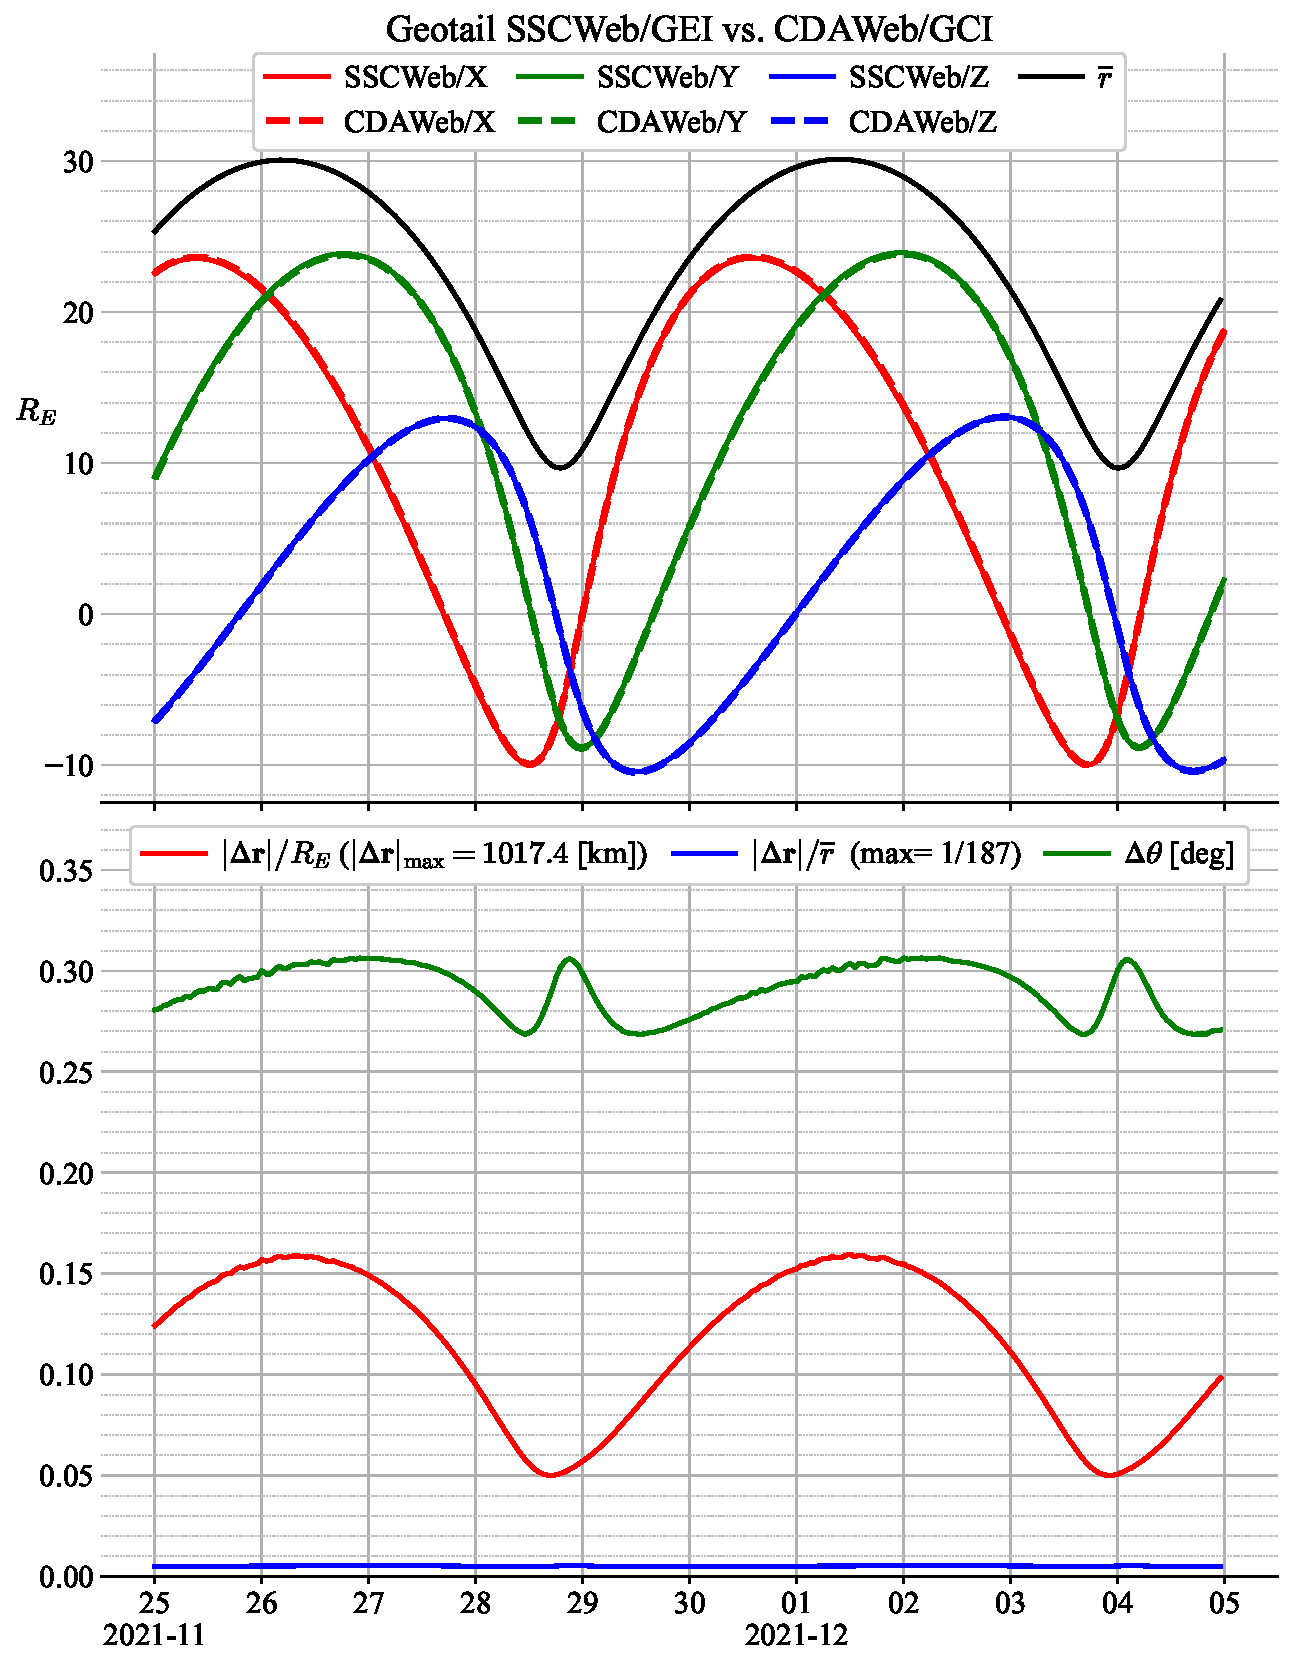
\includegraphics[width=\textwidth]{code/figures/ephemeris/Geotail_SSCWeb-GEI_vs_CDAWeb-GCI.pdf}
     \end{subfigure}
     \begin{subfigure}[b]{0.49\textwidth}
         (b)
         \centering
         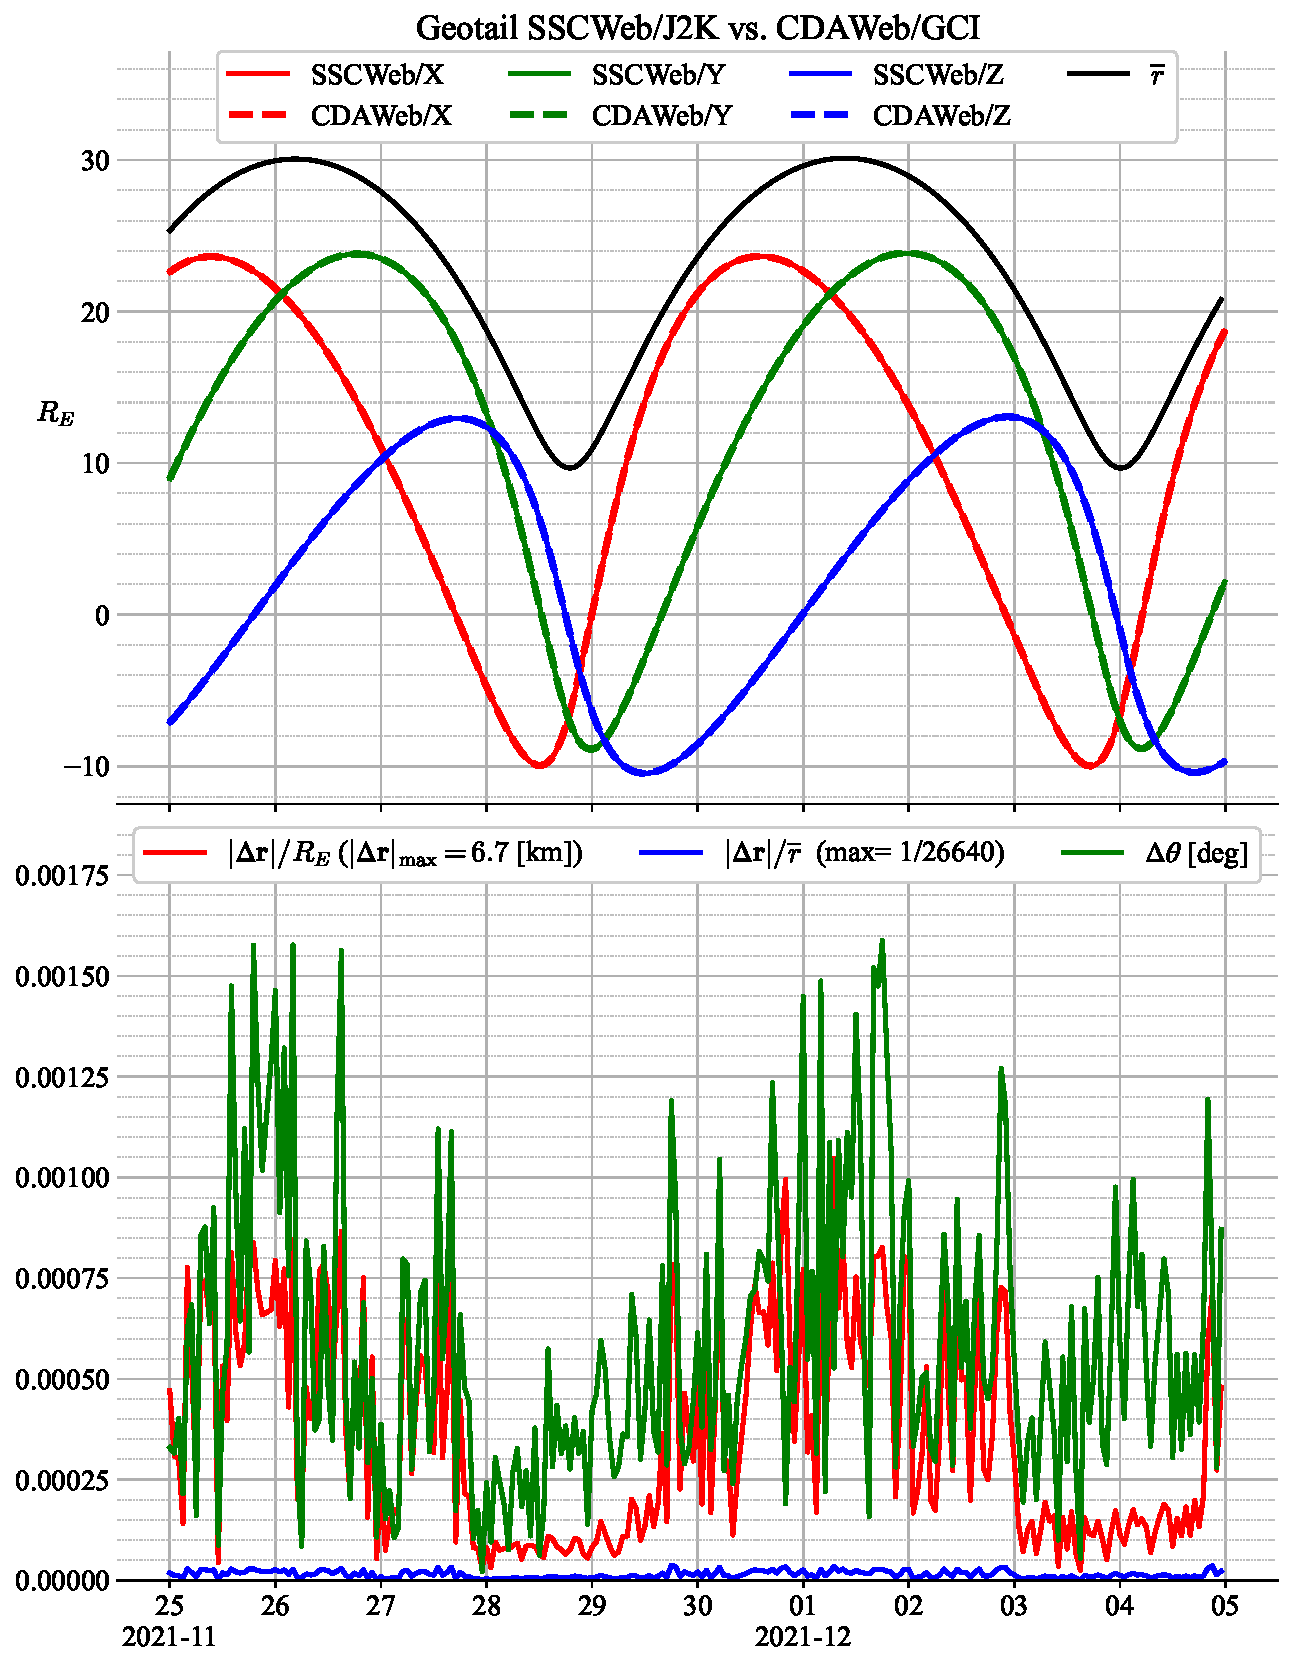
\includegraphics[width=\textwidth]{code/figures/ephemeris/Geotail_SSCWeb-J2K_vs_CDAWeb-GCI.pdf}
     \end{subfigure}
     \par\bigskip\bigskip
     \begin{subfigure}[b]{0.49\textwidth}
         (c)
         \centering
         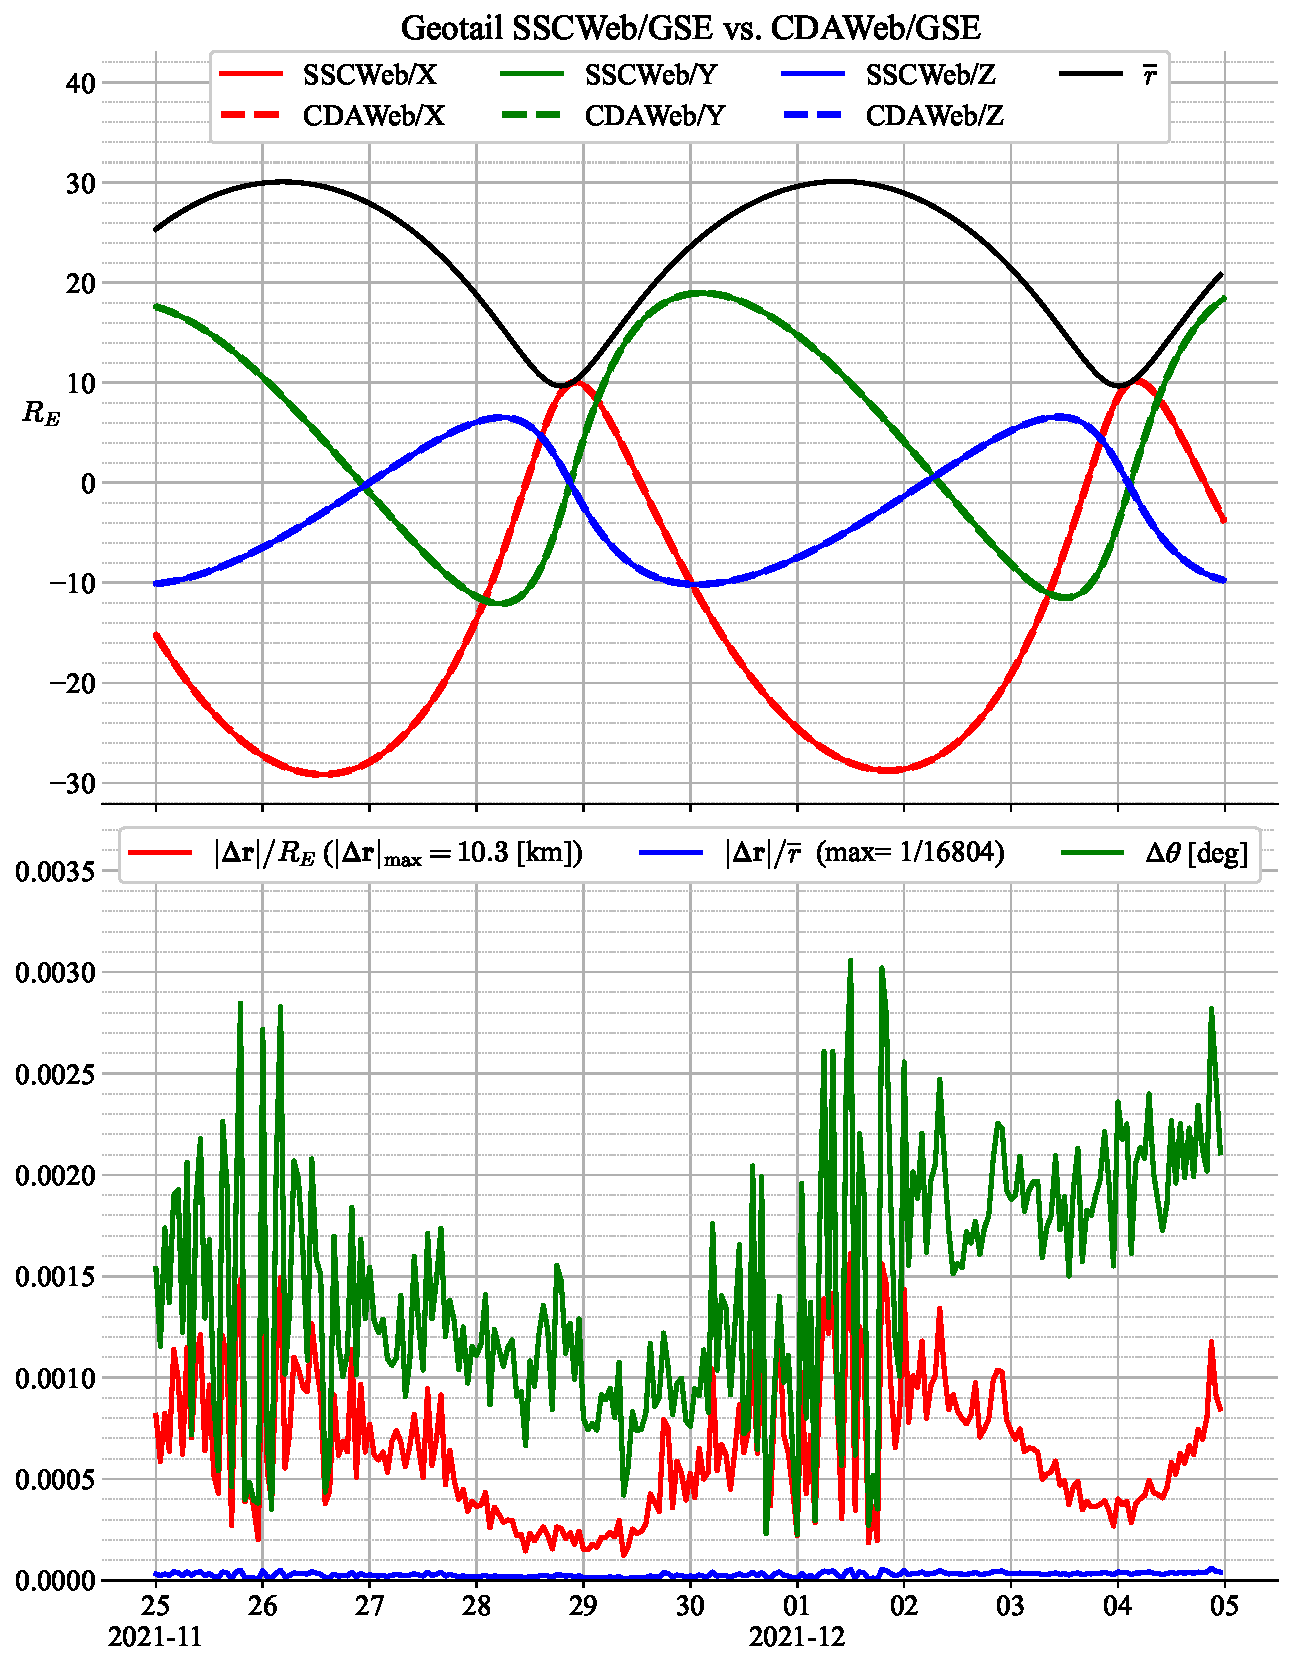
\includegraphics[width=\textwidth]{code/figures/ephemeris/Geotail_SSCWeb-GSE_vs_CDAWeb-GSE.pdf}
     \end{subfigure}
     \begin{subfigure}[b]{0.49\textwidth}
         (d)
         \centering
         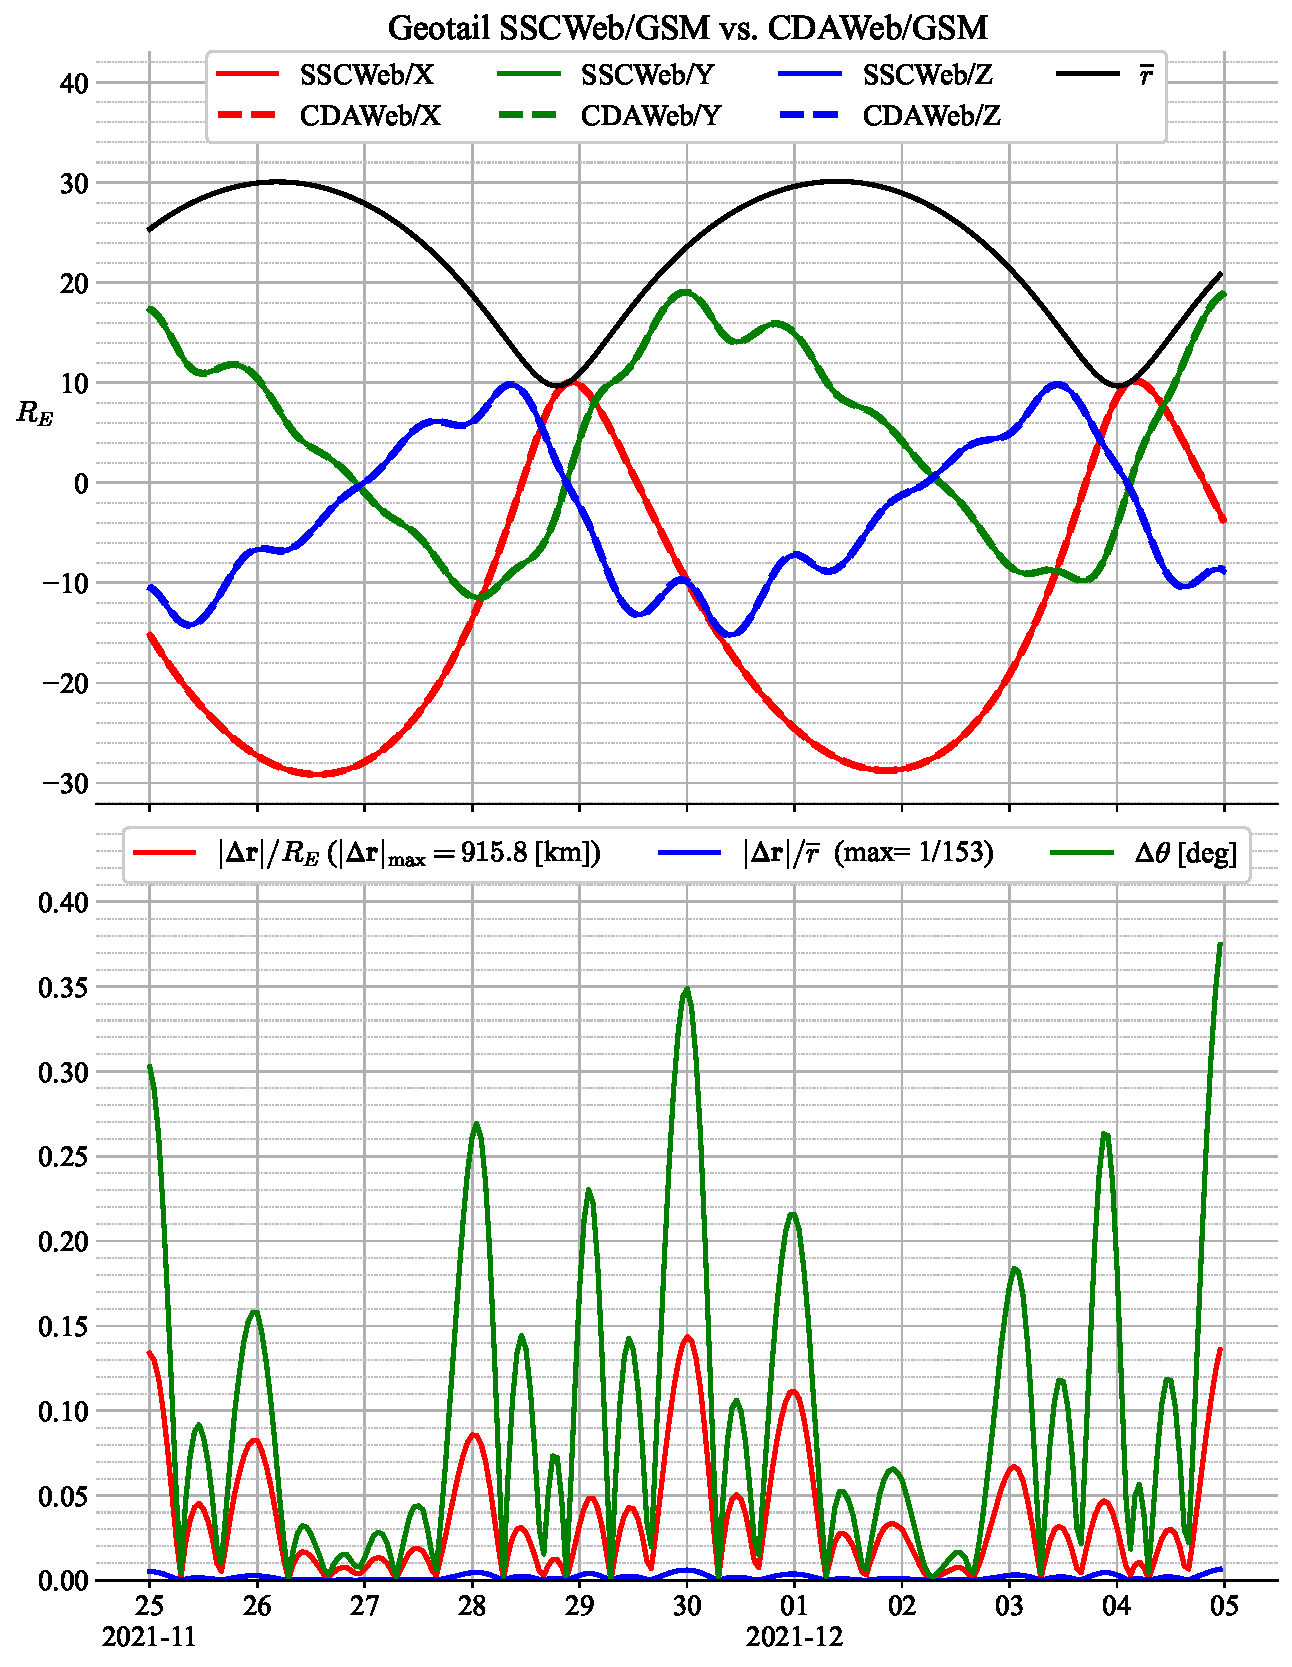
\includegraphics[width=\textwidth]{code/figures/ephemeris/Geotail_SSCWeb-GSM_vs_CDAWeb-GSM.pdf}
     \end{subfigure}
     \caption{Comparison of ephemeris values from SSCWeb and CDAWeb in four different reference systems.}
     \label{fig:geotail}
\end{figure}

\clearpage

\begin{figure}[h]
     \begin{subfigure}[b]{0.49\textwidth}
         (a)
         \centering
         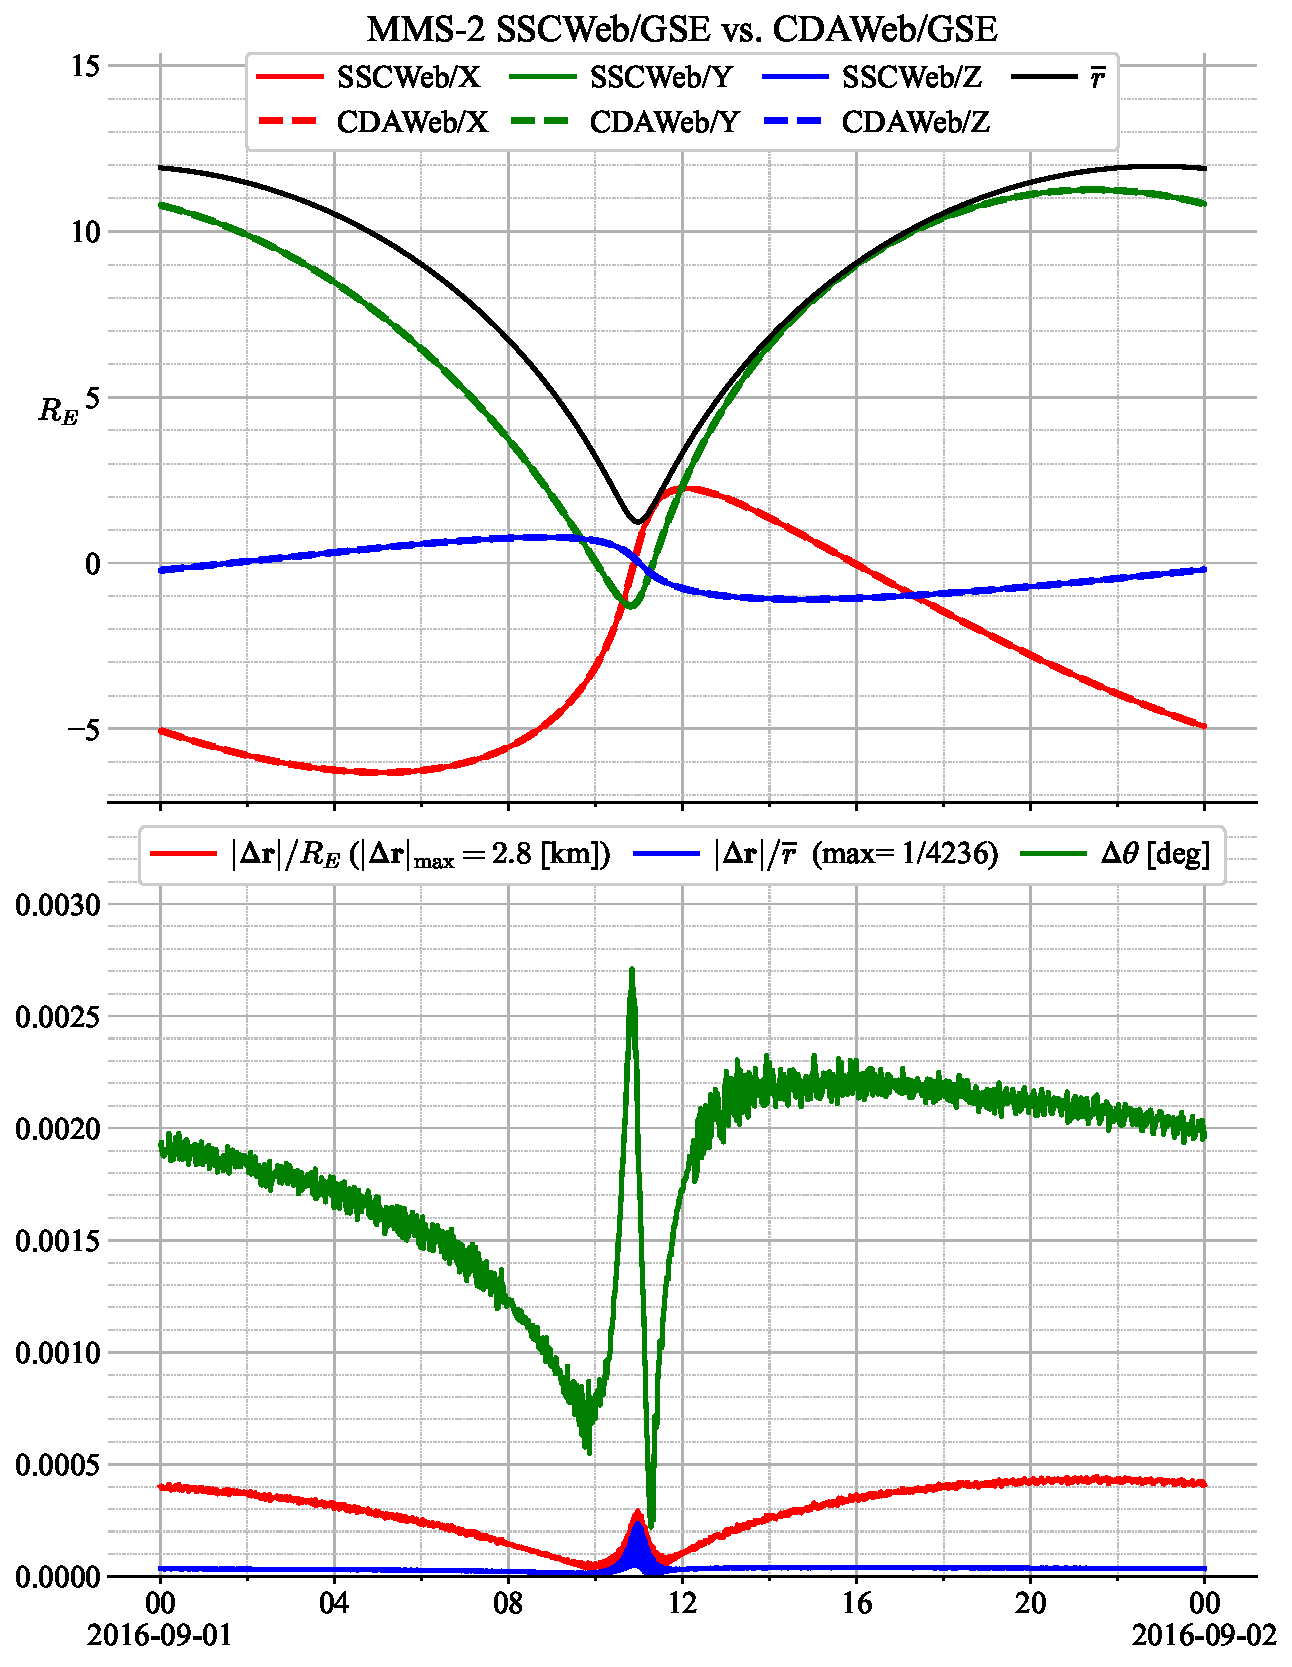
\includegraphics[width=\textwidth]{code/figures/ephemeris/MMS-2_SSCWeb-GSE_vs_CDAWeb-GSE.pdf}
     \end{subfigure}
     \begin{subfigure}[b]{0.49\textwidth}
         (b)
         \centering
         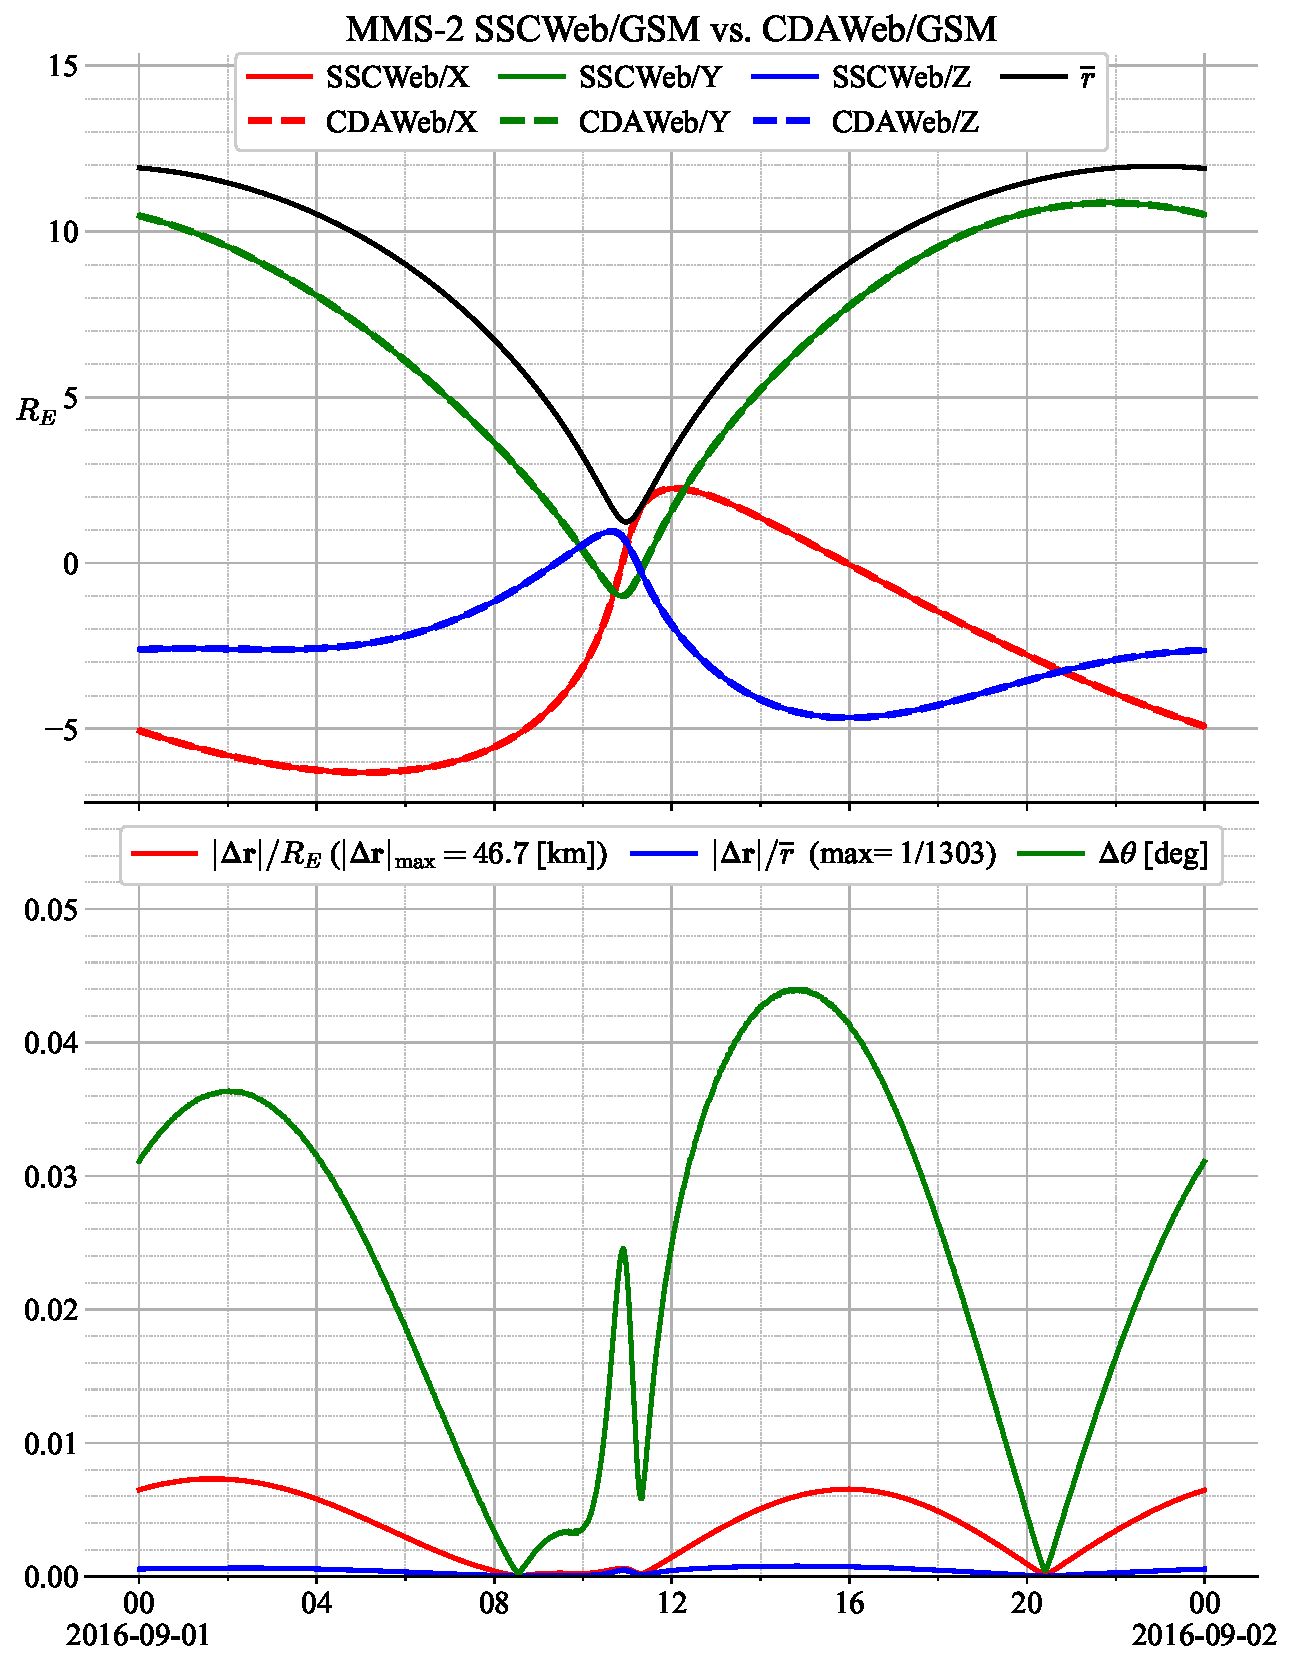
\includegraphics[width=\textwidth]{code/figures/ephemeris/MMS-2_SSCWeb-GSM_vs_CDAWeb-GSM.pdf}
     \end{subfigure}
     \par\bigskip\bigskip
     \begin{subfigure}[b]{0.49\textwidth}
         (c)
         \centering
         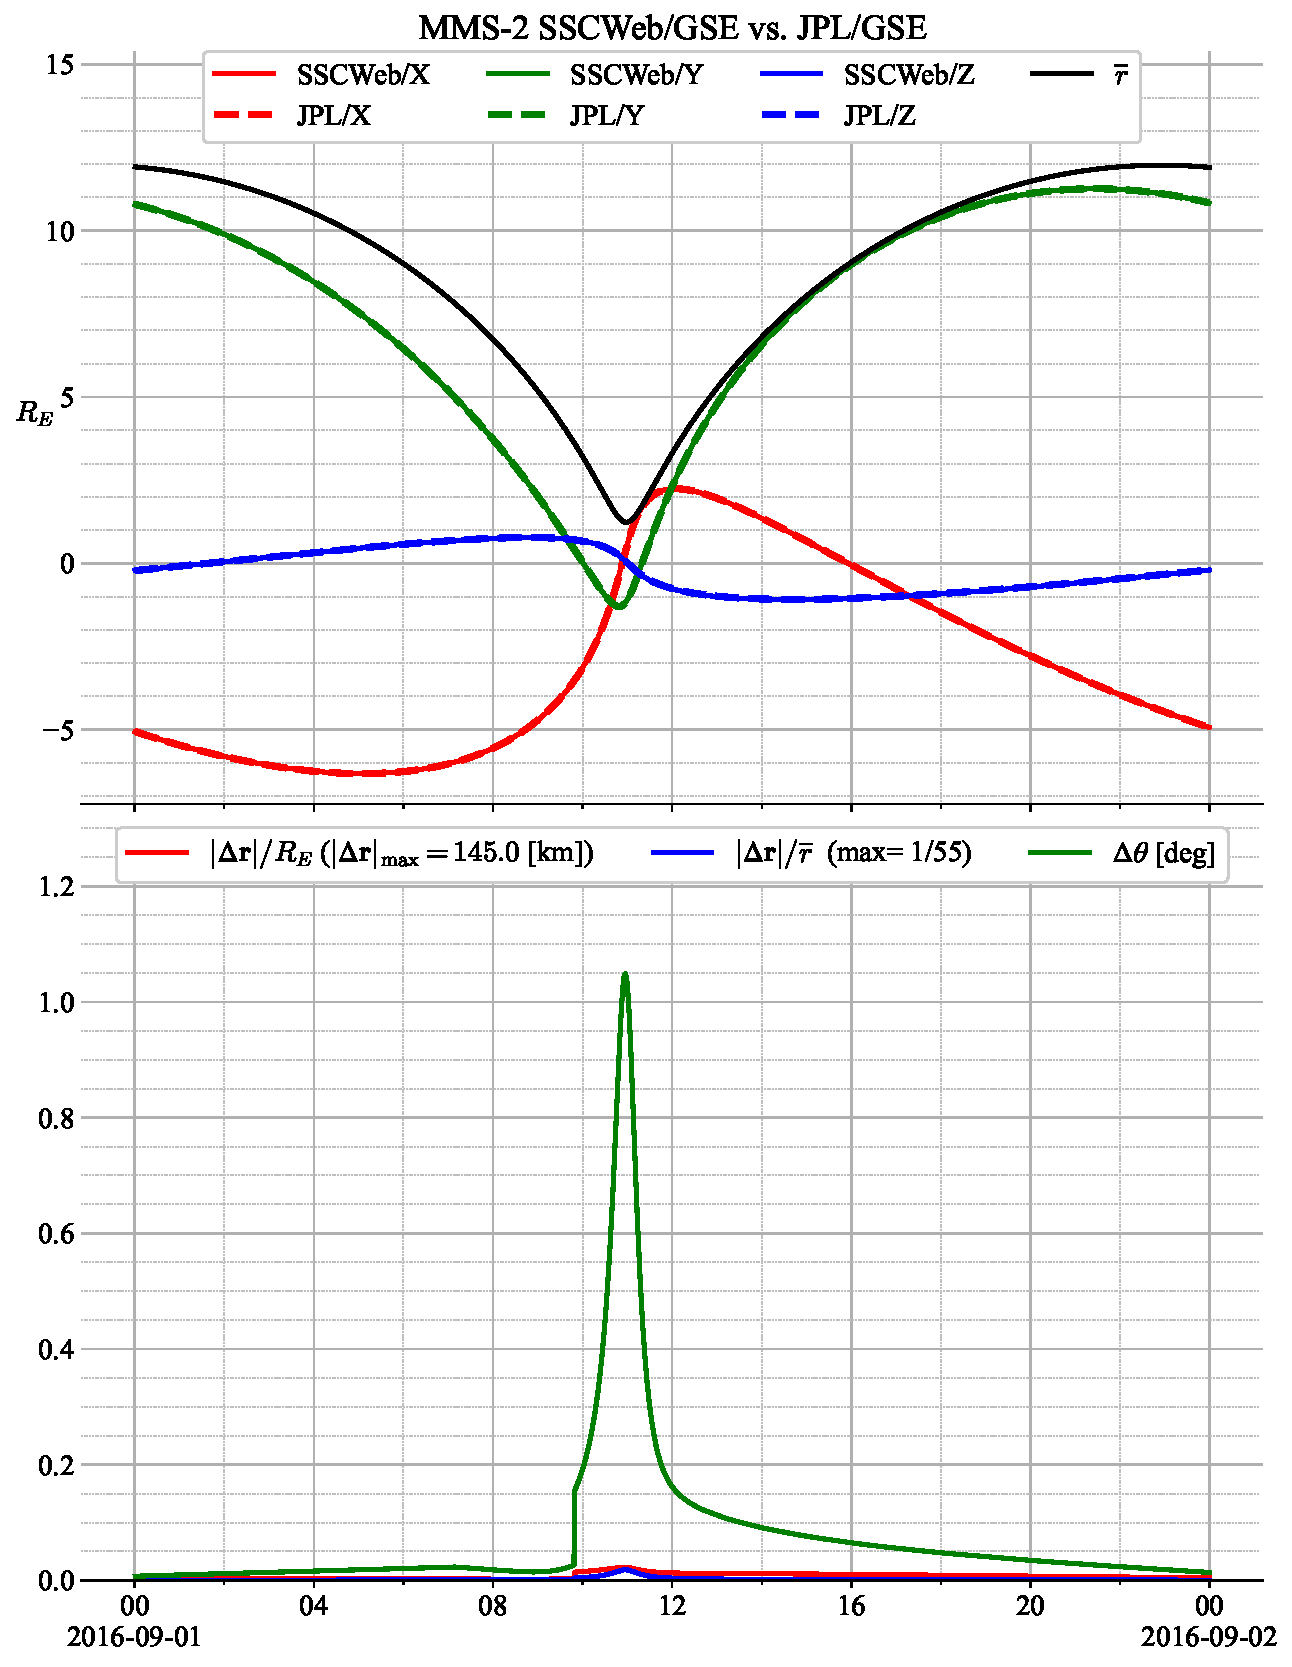
\includegraphics[width=\textwidth]{code/figures/ephemeris/MMS-2_SSCWeb-GSE_vs_JPL-GSE.pdf}
     \end{subfigure}
     \begin{subfigure}[b]{0.49\textwidth}
         (d)
         \centering
         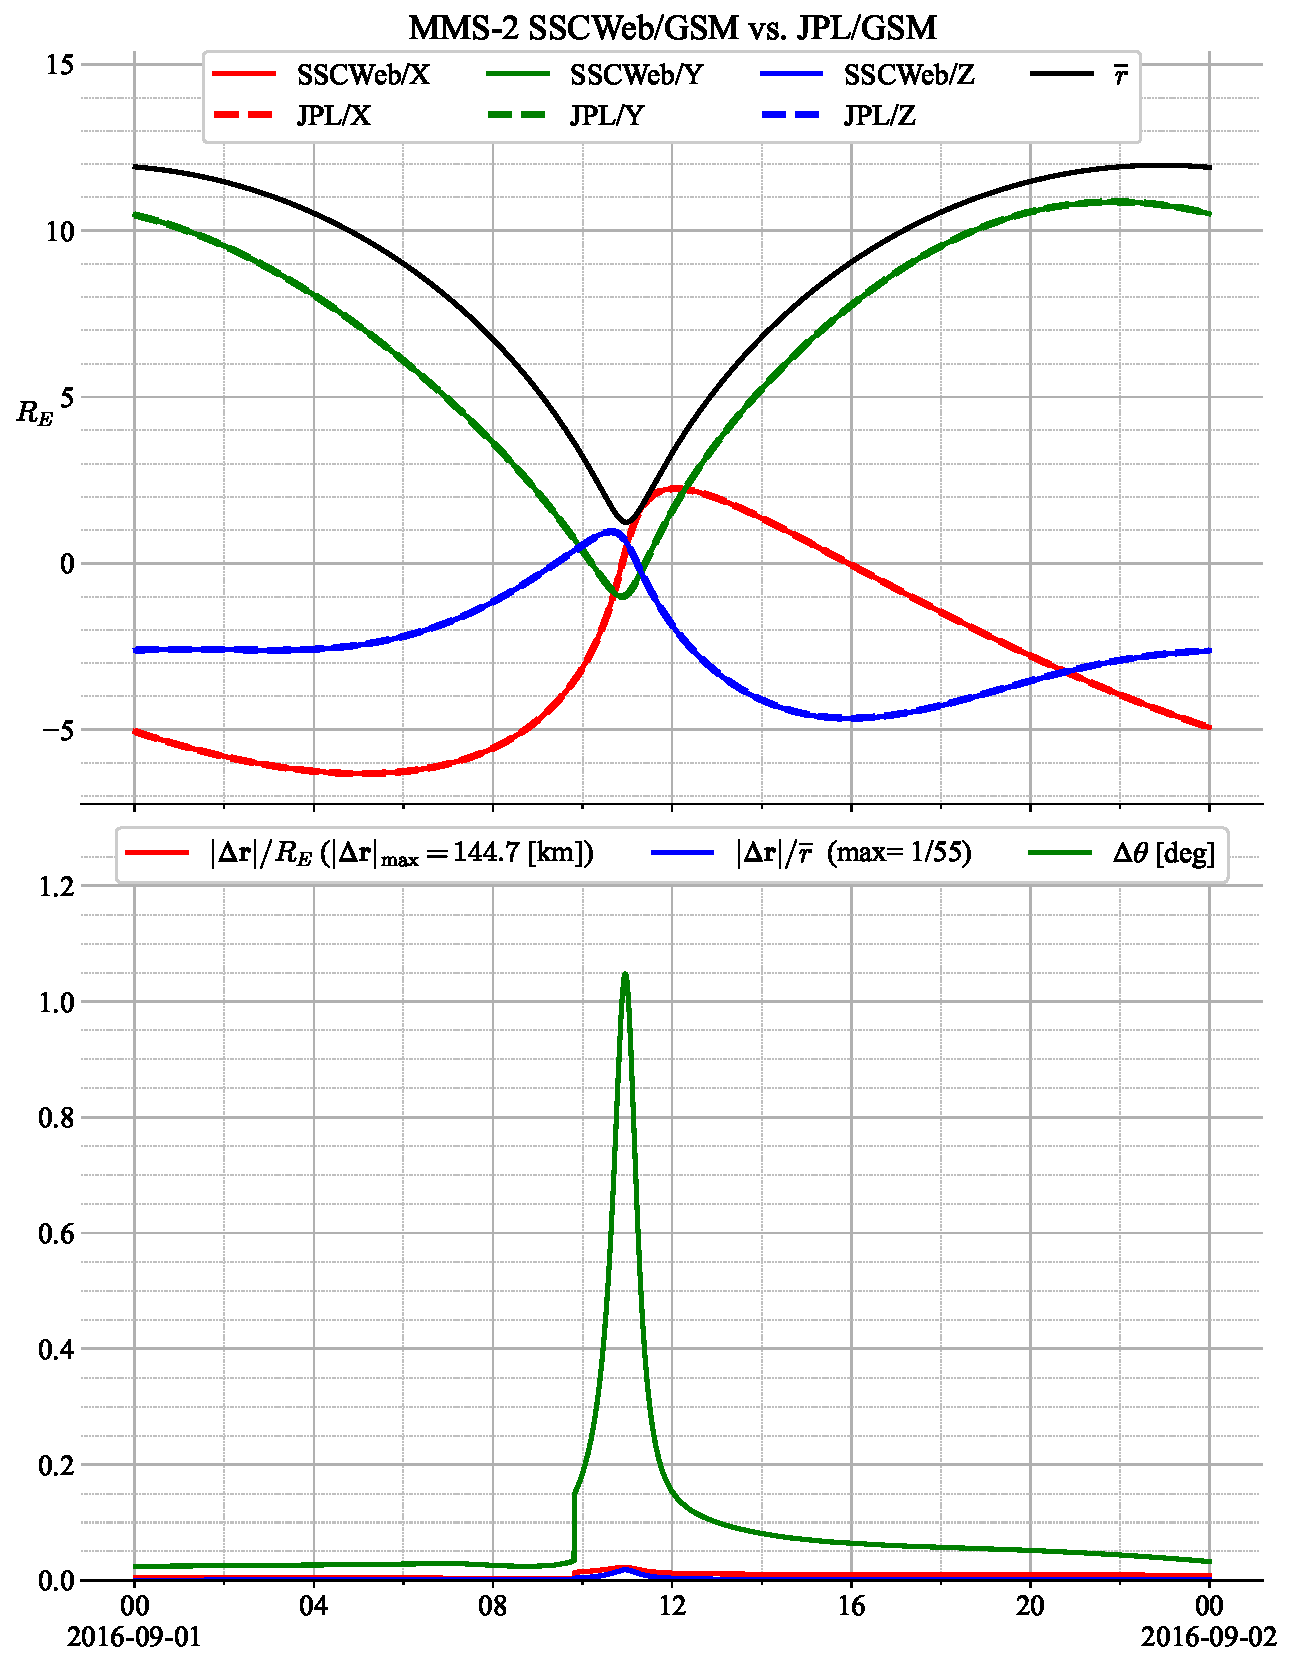
\includegraphics[width=\textwidth]{code/figures/ephemeris/MMS-2_SSCWeb-GSM_vs_JPL-GSM.pdf}
     \end{subfigure}
     \caption{Comparison of ephemeris values from (a)--(b)  SSCWeb and CDAWeb; (c)--(d) SSCWeb and JPL Horizons in two different reference systems.}
     \label{fig:mms-2}
\end{figure}

\clearpage

%These calculations were based on ... ISTP software. The results from \citeA{SSCWeb} were obtained using its web interface, which dynamically computes results based on ...

%\todo[inline]{Finish after browsing code, which is private Google Drive folder 2023_STCT_NASA}.

%Another recommendation: service provides links to software used (sometimes not possible)

\subsection{Software}
\label{sect:comparisons_software}

In this section, we compare reference frame calculations using the following software packages. 

\begin{itemize}
    \item \texttt{Geopack-2008} double precision (\citeA{Tsyganenko2008}; labeled as \texttt{geopack\_08\_dp} in the figures in this section), a Fortran library that was upgraded from earlier versions to support calculations using 64--bit floating point values.
    % Use True of date GEI
    \item \texttt{PySPEDAS} 1.7.28, which uses transformation code derived from the IDL version of \texttt{PySPEDAS} \cite{Angelopoulos2024IDL}, which in turn used code from the \texttt{ROCOTLIB} Fortran \cite{ROCOTLIB} library, which was used for data from the Cluster spacecraft mission \cite{ClusterTools1993}.
    \item \texttt{SpacePy} 0.0.6, which has an option to use the \texttt{IRBEM} Fortran library (\citeA{IRBEM2022}; labeled as \texttt{spacepy-irbem}) or a native Python implementation (\texttt{spacepy}) of the transforms.
    \item \texttt{SpiceyPy} 6.0.0 is a Python wrapper for the SPICE toolkit. Two versions of SPICE kernel files were used, indicated by \texttt{spicepy1} and \texttt{spicepy2}. \texttt{spicepy1} was used for reference frame transforms for the Van Allen Probes mission. \texttt{spicepy2} had an update to the \texttt{MAG} frame, which used a more recent version of the IGRF model \cite{Alken2021} to determine the Earth's magnetic dipole orientation.
    \item \texttt{SunPy} version 7.0.0
\end{itemize}

Figure~\ref{fig:angles} compares the angles between the $Z$ axis of select coordinate frame pairs. The average of the absolute value of the differences with respect to \texttt{geopack\_08\_dp} ranges from $4\cdot 10^{-7}$ to $1\cdot 10^{-2}$ degrees; the values for each library are given in the legend in the middle panel of each subplot. These values can be used as an uncertainty estimate when comparing data transformed using different software libraries.

The maximum absolute differences shown in the bottom panels of the subplots in Figure~\ref{fig:angles} are smaller than those found when comparing ephemeris values in section~\ref{sect:comparisons_ephemeris}. The choice of which library to use as a baseline for this comparison is arbitrary; in general, we are interested in the maximum differences among the libraries, which is displayed in the lower panel of each subplot.

The bottom panels of Figure~\ref{fig:angles}a--c shows that the maximum difference between the libraries for the \texttt{GEO}/\texttt{GSE} is ${\sim}0.02^\circ$,  \texttt{GEO}/\texttt{GSM} is ${\sim} 0.03^\circ$, \texttt{GEO}/\texttt{GSM} is ${\sim}0.04^\circ$, all of which are comparable to the average angular change in Earth's dipole $Z$ axis of ${\sim}0.04^\circ$ per year.

%Figure~\ref{fig:angles}d s

We have also performed coordinate transforms using the \citeA{SSCWebCoordinateCalculator} coordinate calculator web service. However, this service only outputs values to two decimal places, which leads to angular differences of $0.3^\circ$. These values are not plotted so that the library differences are clearly visible.

\begin{figure}[htb]
     \begin{subfigure}[b]{0.49\textwidth}
         (a) $\angle (Z_{GEO}, Z_{GSE})$
         \centering
         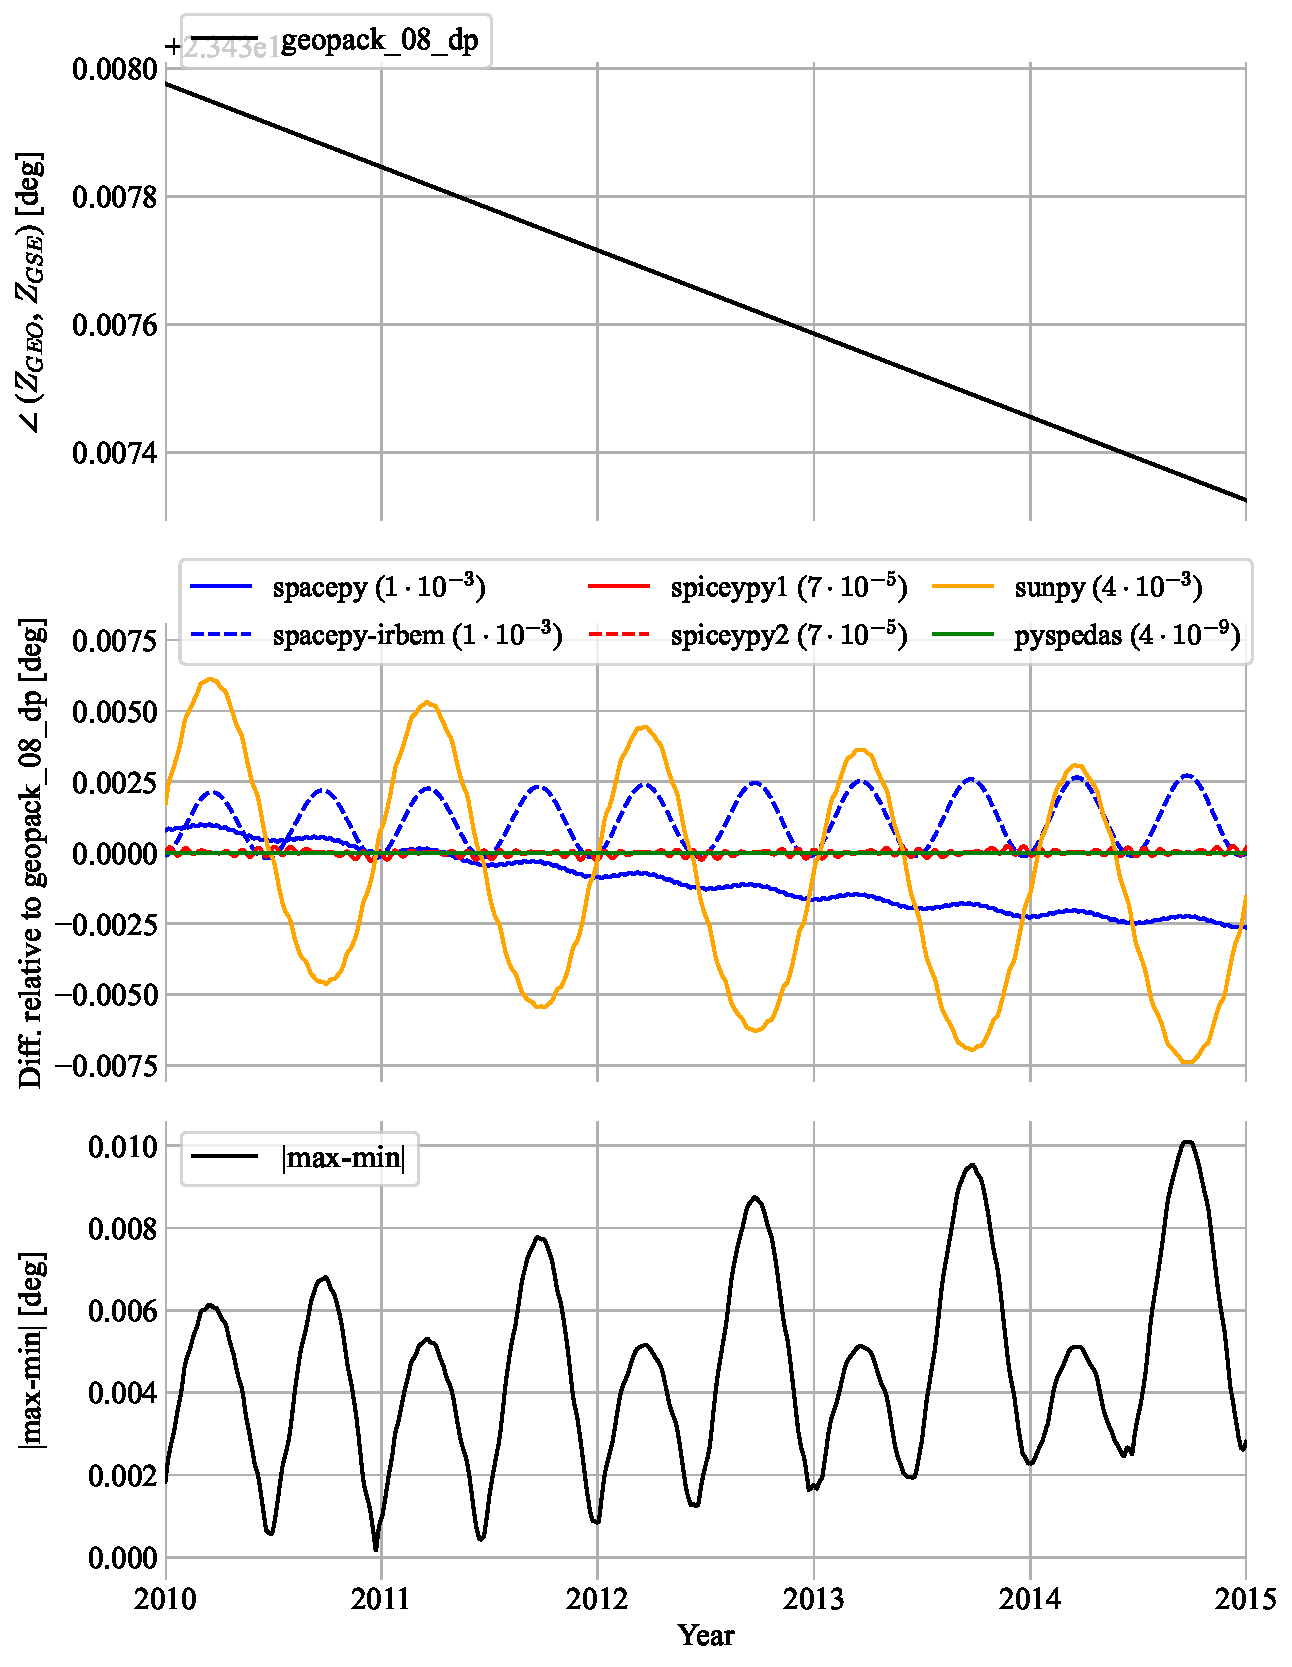
\includegraphics[width=\textwidth]{code/figures/angles/z-delta=1days_20100101-20150101/GEO_GSE.pdf}
     \end{subfigure}
     \begin{subfigure}[b]{0.49\textwidth}
         (b) $\angle (Z_{GEO}, Z_{GSM})$
         \centering
         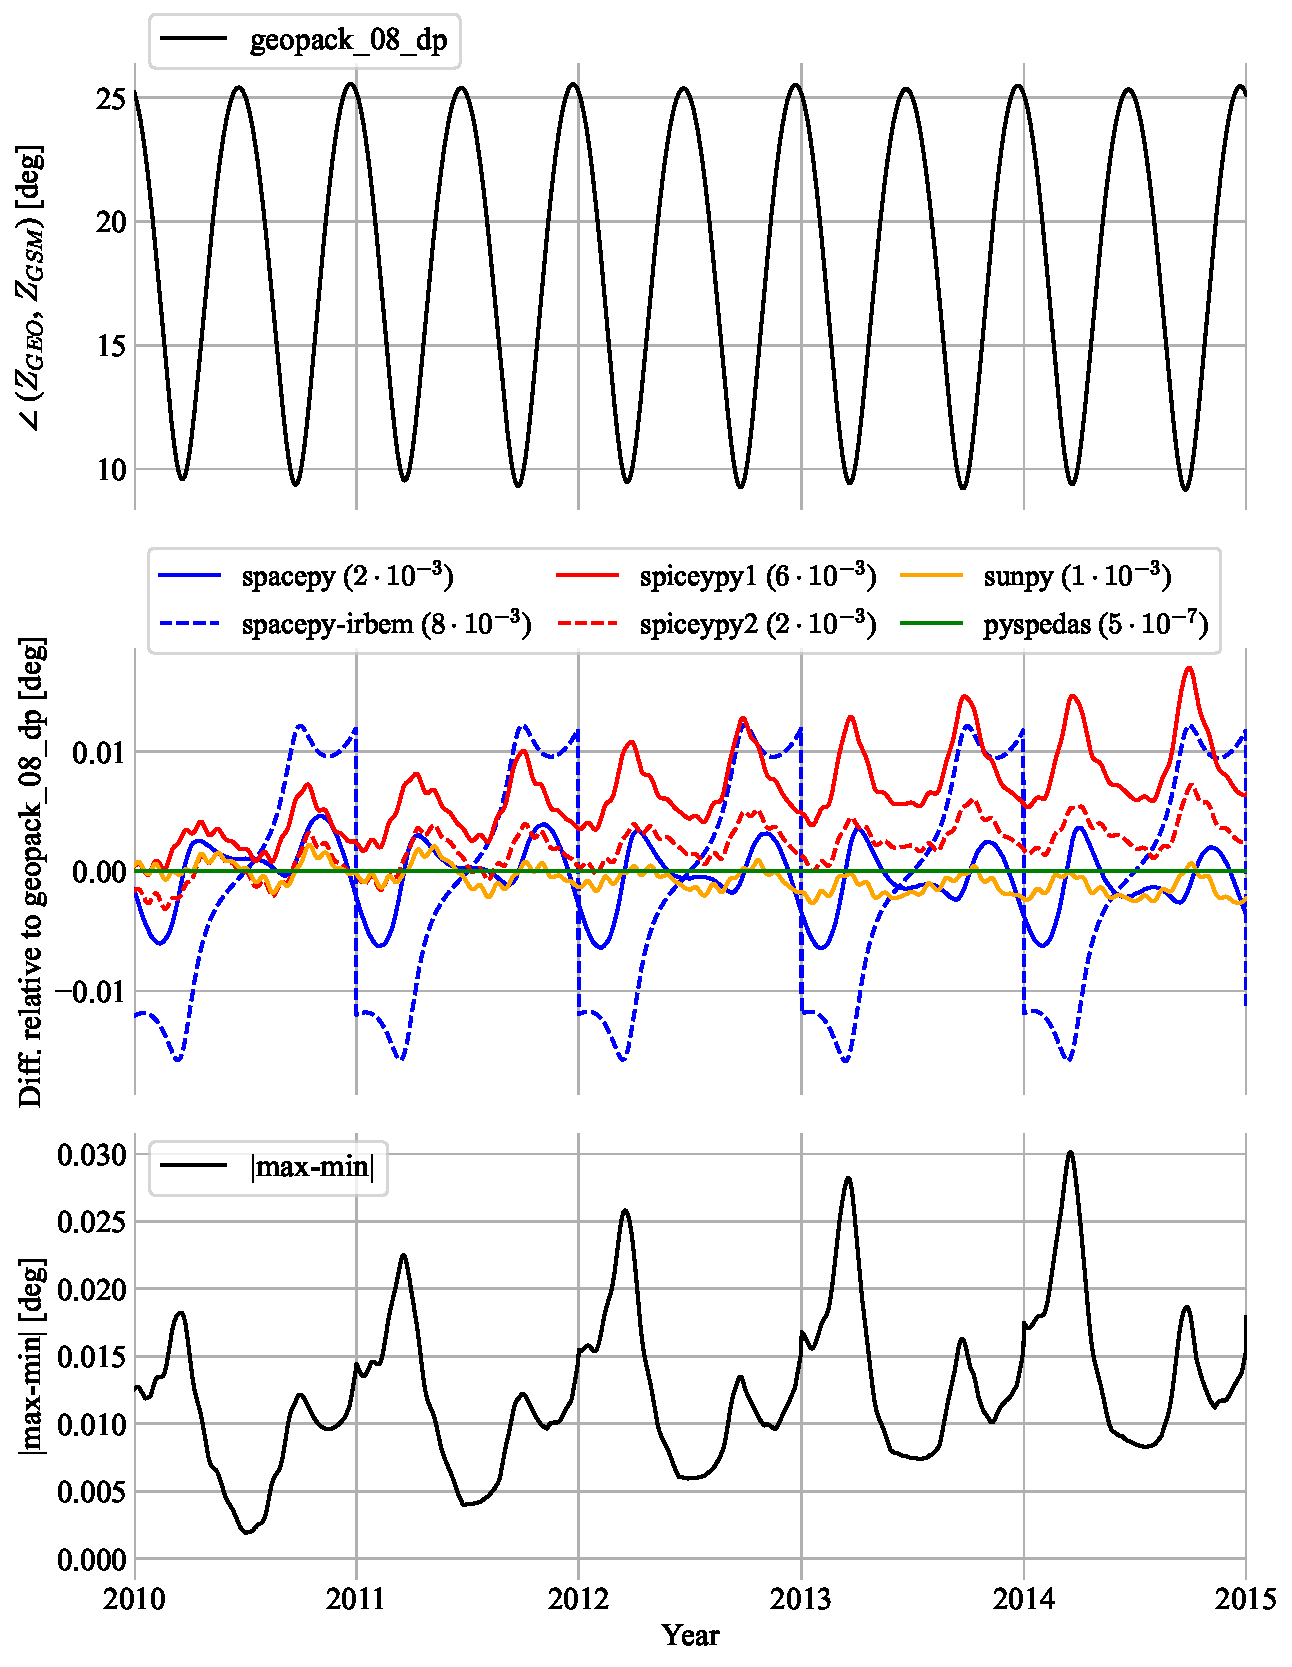
\includegraphics[width=\textwidth]{code/figures/angles/z-delta=1days_20100101-20150101/GEO_GSM.pdf}
     \end{subfigure}
     \par\bigskip\bigskip
     \begin{subfigure}[b]{0.49\textwidth}
         (c) $\angle (Z_{GSE}, Z_{GSM})$
         \centering
         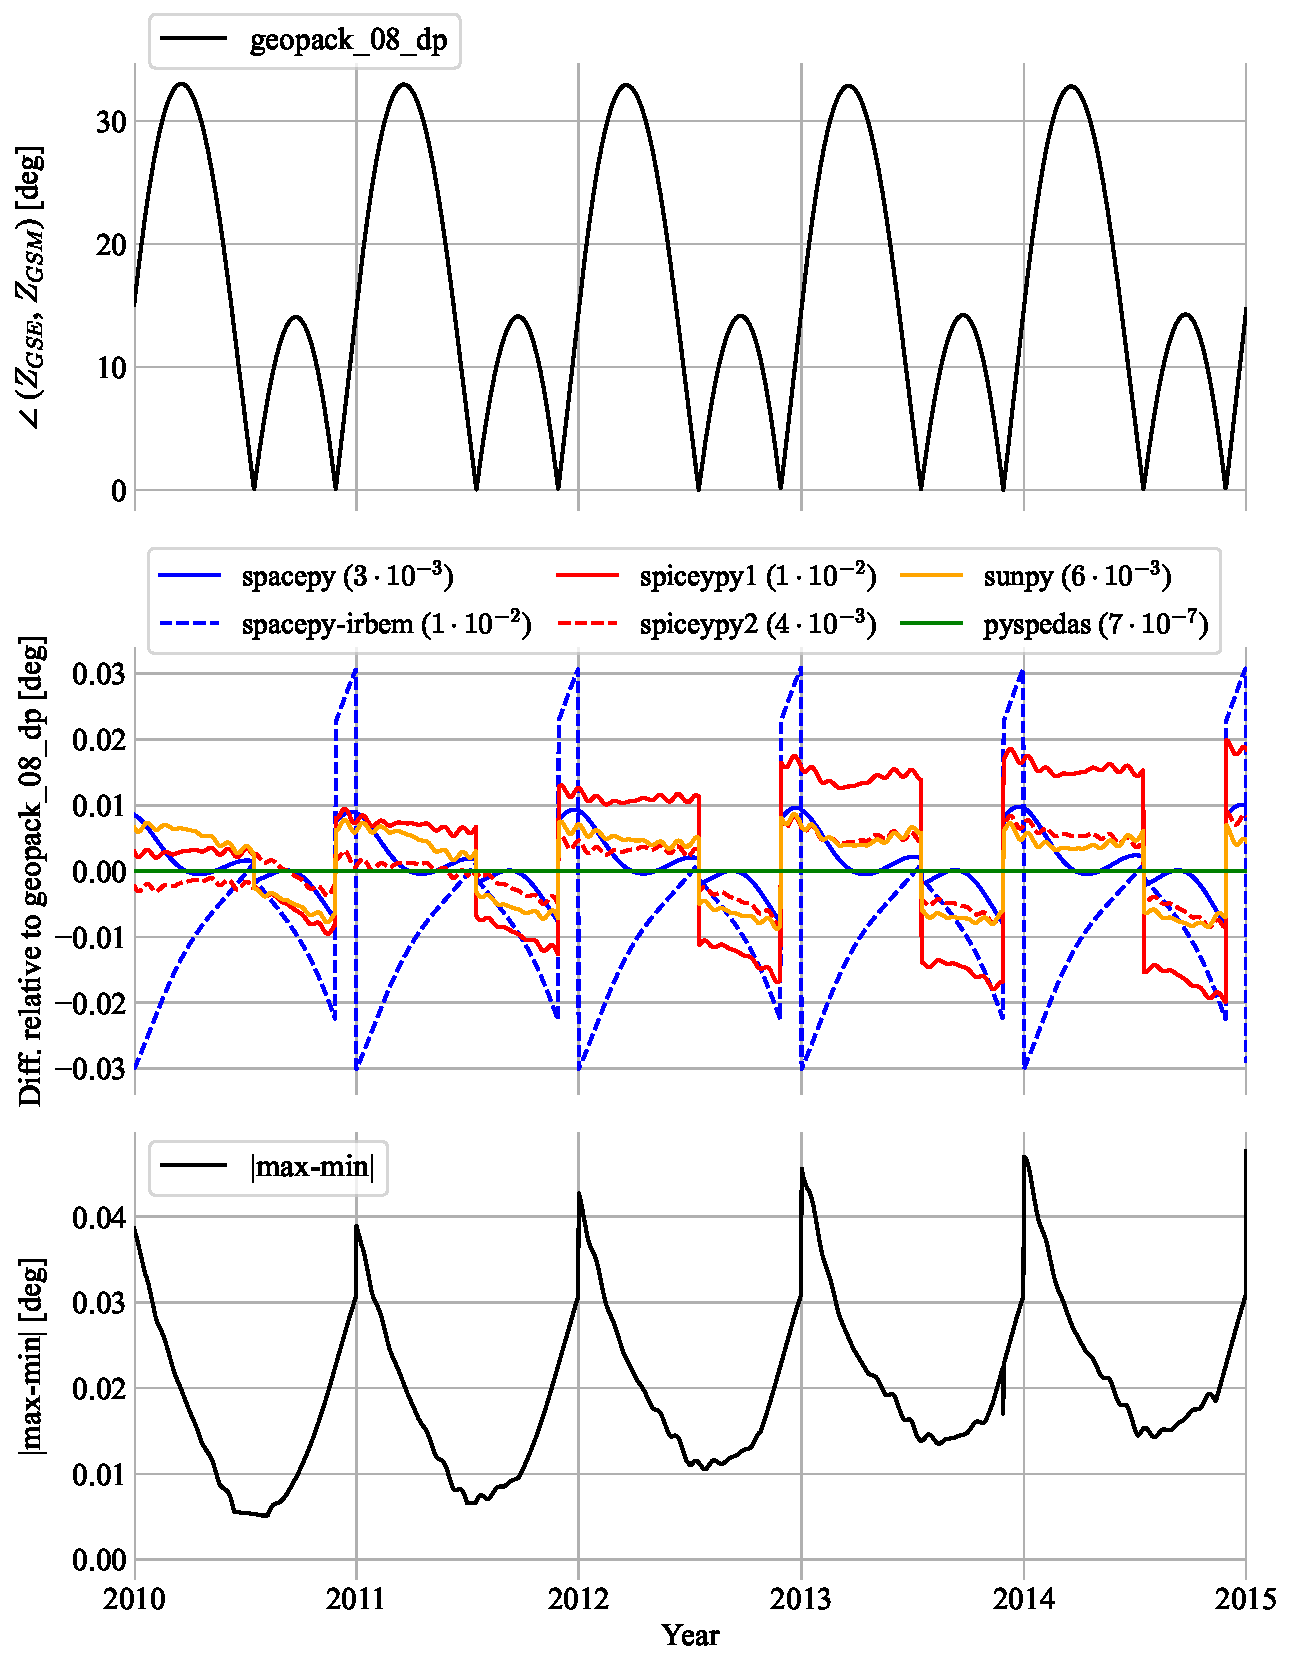
\includegraphics[width=\textwidth]{code/figures/angles/z-delta=1days_20100101-20150101/GSE_GSM.pdf}
     \end{subfigure}
     \begin{subfigure}[b]{0.49\textwidth}
         (d) $\angle (Z_{MAG}, Z_{GSM})$
         \centering
         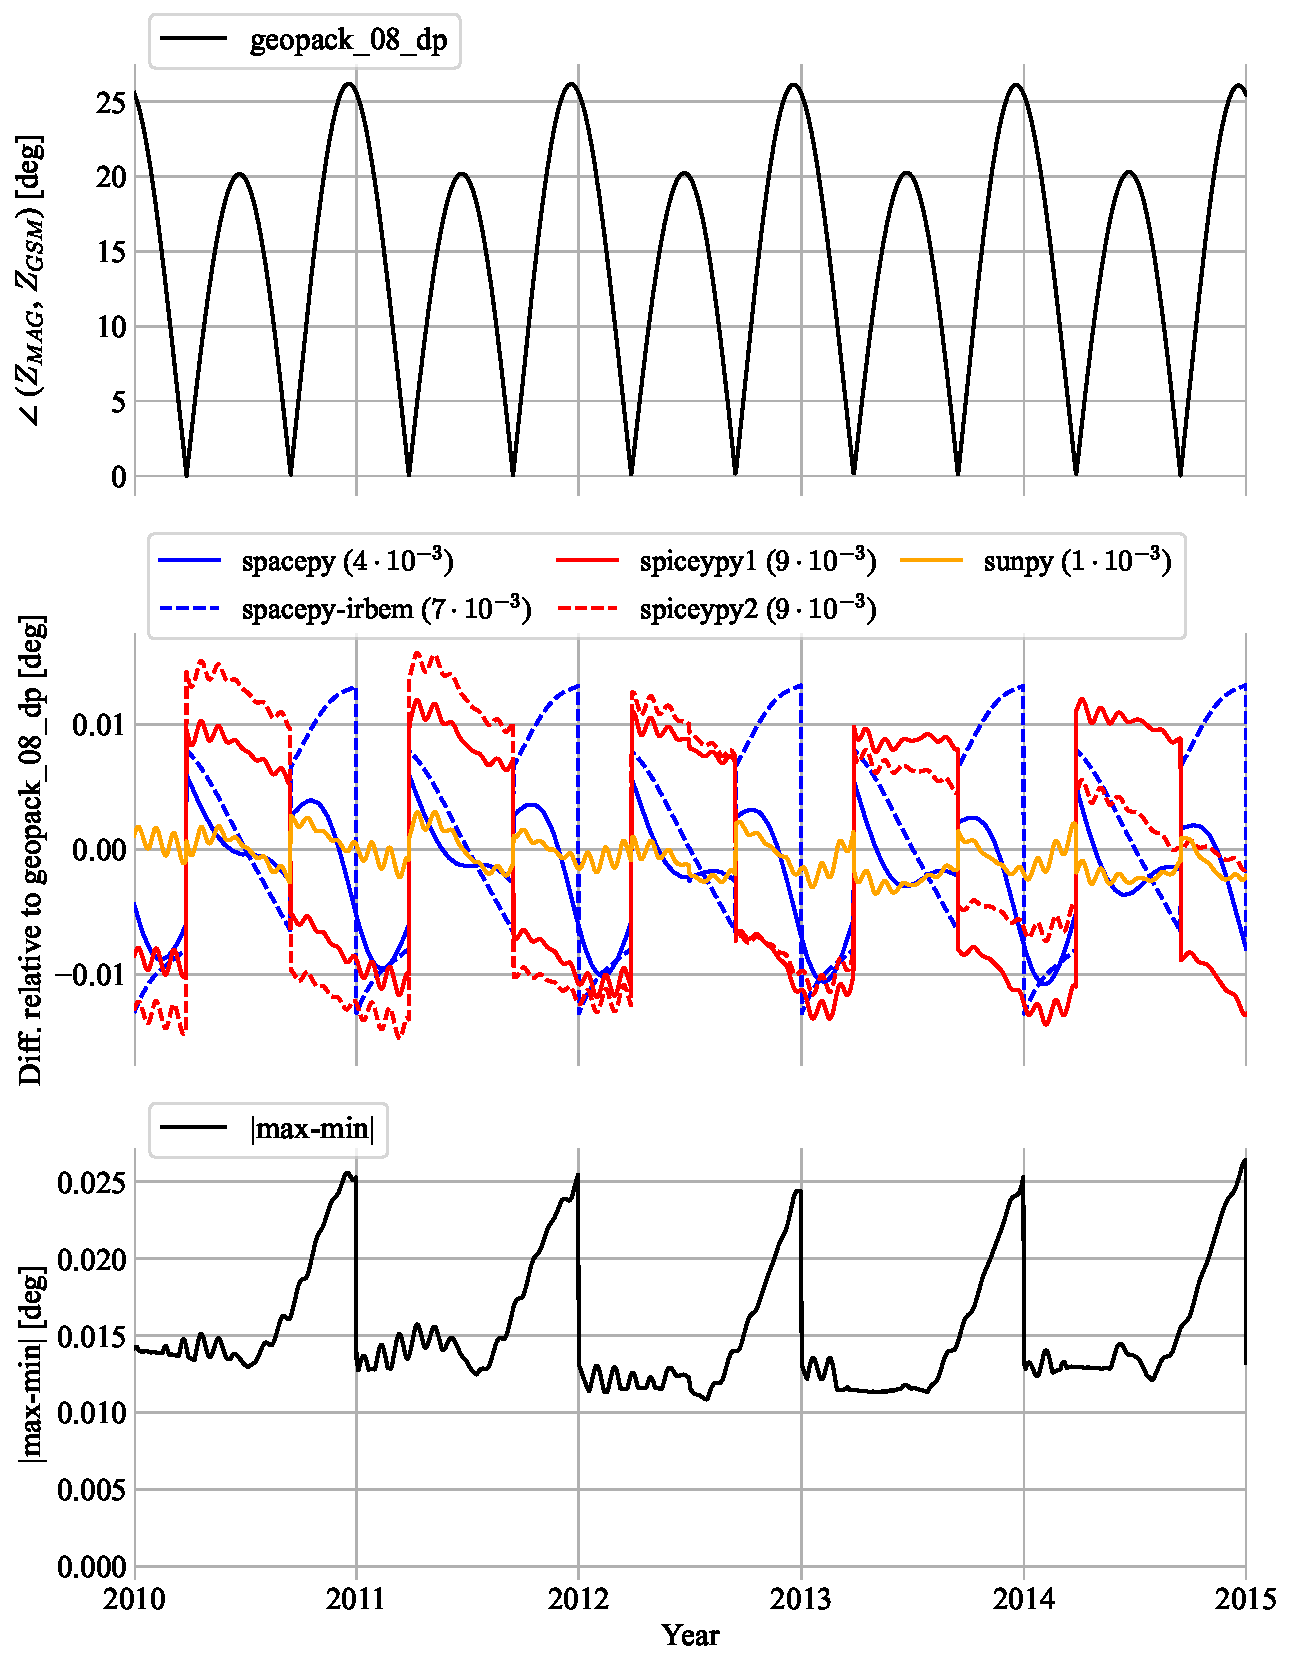
\includegraphics[width=\textwidth]{code/figures/angles/z-delta=1days_20100101-20150101/MAG_GSM.pdf}
     \end{subfigure}
     \caption{Angles between $Z$ axes in select coordinate frames. In the top panels of each subplot, the notation $\angle (Z_A, Z_B)$ means the angle between the $Z$ axis of coordinate frame $A$ in coordinate frame $B$ and the $Z$ axis of coordinate frame $B$. At this scale, the differences between the libraries are not visible. The middle panel of each subplot shows the difference in the computed angles in the top panel with respect to \texttt{geopack\_08\_dp}, with the average of the absolute value of each line shown in parentheses. In subplot (a), the values for \texttt{spicepy1} and \texttt{spiceypy2} are identical. The bottom panels show the maximum absolute value of the differences in the middle panel.}
     \label{fig:angles}
\end{figure}

\clearpage

\section{How transform information is created for spacecraft missions}
\label{sect:missions}

Archival data for space physics spacecraft missions typically include vector measurements in multiple reference frames. For NASA missions, the archival data products are delivered to the Space Physics Data Facility \cite{SPDF}. Modern missions typically take one of two approaches: (a) A mission operations team develops SPICE kernels for select space physics reference frames, and SPICE software is used for the transforms; or (b) A non--SPICE software library is used for the transforms, for example, \texttt{ROCOTLIB} and \texttt{SpacePy}. 

There is a significant overlap in effort --- typically, a scientist familiar with space physics reference systems, but not their many options for implementation, will use available software or SPICE kernels and develop tests. 

As noted in the conclusions, this effort to develop and verify transforms for variables into different reference frames would not be necessary if either a database of transform matrices or versioned SPICE kernels were available that were accepted as a community standard.

For the SSCWeb data service \cite{SSCWeb}, which provides spacecraft ephemeris, three approaches have been taken in order of priority (see \citeA{SSCWebProvenance} for a table indicating which approach was taken and provenance):

\begin{enumerate}
    \parskip 0.1in 

    \item Mission--developed SPICE kernels for ephemeris are ingested and archived. The \texttt{GEI} ephemeris--related SPICE kernel information is used to generate its \texttt{J2000} ephemeris. Then International Solar-Terrestrial Physics--era (ISTP; \citeA{ISTP2025}) software is used to compute ephemeris in different coordinate frames, including \texttt{GEI}, \texttt{GEO}, \texttt{GM}, \texttt{GSE}, \texttt{GSM}, and \texttt{SM}. The ISTP software uses proprietary information needed for the reference frames (such as the position of the Sun) calculated by GSFC's Flight Dynamics Facility, FDF.  This approach is only used on ISTP--era missions, e.g., ACE, Polar, Wind, and Geotail.

    \item A \texttt{GEI} ephemeris--related variable in archival CDF files ingested from the mission database is used. ISTP--era software is used to compute ephemeris in different coordinate frames; if the CDF files contain ephemeris in reference frames other than the \texttt{GEI}--related frame, they are not used.

    \item If SPICE kernels or other mission--computed values are not available, TLE (Two-Line Element) files are obtained from NORAD (North American Aerospace Defense Command), and a translation of the C NORAD library to Pascal \cite{NORADSGP4c} is used to compute ephemeris in \texttt{TEME} (True Equator, Mean Equinox). Often, TLEs are used at the start of the mission, and a switch is made to approaches 1 or 2 as information becomes available.
    
    %(special arrangement with NORAD regarding military s/c),

    % Hoots and Roehrich [1988]: ``The most important point to be noted is that not just any prediction model will suffice. The NORAD element sets are ``mean" values obtained by removing periodic variations in a particular way. In order to obtain good predictions, these periodic variations must be reconstructed (by the prediction model) in exactly the same way they were removed by NORAD." Hence the NORAD SGP4 and SDP4 orbit predictor models give the best orbit predictions using TLEs. Felix R., Hoots, F. R., R. L. Roehrich, SPACETRACK REPORT NO. 3 Models for Propagation of NORAD Element Sets, December 1 980 Package Compiled by TS Kelso 31 December 1988.
\end{enumerate}


%Albert: ESA defined \texttt{HEE} differently from NASA in Solar Orbiter SPICE kernel see \texttt{SOLO\_HEE\_NASA} and \texttt{SOLO\_HEE} in \url{https://spiftp.esac.esa.int/data/SPICE/SOLAR-ORBITER/kernels/fk/solo_ANC_soc-sci-fk_V02.tf}

%TLEs are from CelesTrek and can't be distributed. Are public TLE repos, but are they the same?

%Discuss fact that TLEs, location info provenance may never be available, but should be aware of how it is done.

% Need to recommend ISTP name convention for GEI_2000 varaibles in CDF files. Getting agreement on names not possible, but could use attribute.

%https://sscweb.gsfc.nasa.gov/sscweb_data_provenance.html the SPICE kernels are obtained by ingest of directories. "Would be nice if required data delivery was SPICE kernels instead of being ancillary". In some cases, missions does provide SPICE kernels, in which case they use TLEs. TLEs less accurate than SPICE kernels and can't to predict as far out as in SPICE (which can use full time history).

%Ivar: given spk file with positions in gei_2000. How they did transforms to get there is not documented ... (e.g., from gps to gei_2000). Ivar gets csv values from Millenum xyz, vx, vy, vz (state information).

%Tracers location is determined by GPS from Millenium space systems (running moc) then they compute GPS to GEI (use GEI_2000) and deliver to mission.

\section{Summary and Recommendations}
\label{sect:conclusions}

%Comment on definition of $R_E$ and problem with providing measurements in terms of $R_E$.

In this section, we provide recommendations to address the issues identified in this article.

\subsection{Standards for Reference System and Frame Definitions}
\label{sect:standard-for}

As defined in section~\ref {sect:terminology}, an {\it ideal reference system} is a general description of a reference frame that lacks key details necessary for its implementation. Examples were provided where the \texttt{GEI} acronym had different expansions, and different acronyms were identified as equivalent to one another.
  
The next level of specificity relative to an ideal reference system is a {\it reference system}, which defines constants, models, and algorithms used to transform between observable quantities and reference data. 

Finally, a {\it reference frame} is a realization of a reference system based on measurements that are used to determine the free parameters the models specified in a reference system model. 

A community--developed standard should be created for acronyms and definitions. The standard should provide abbreviation/definition pairs for commonly used space physics ideal reference frames. Associated with each ideal reference frame definition, there should be at least one reference system abbreviation/definition pair; if multiple reference systems are in common use, they should have their definition and way of being referred to. For each reference system, there should be at least one reference frame abbreviation/definition.
%There are two community--developed standards with ideal reference frame definitions: IVOA [Ref] and SPASE [Ref].

\subsection{Reference Frame Standard Dataset}
\label{sect:reference-dataset}

For a given transform between reference frames, a transformation matrix at a specific instant in time (or, equivalently, rotation angles or quaternions) relative to a base reference frame is required. We also note that implementing transforms requires technical expertise in software and maintenance, such as updating parameters in reference frames, verifying calculations, and documenting changes. Although providing a software version allows for reproducibility in principle, in practice, not all users will be familiar with the cited software, and in the long term, the software may not be maintained, or it may be difficult to install and use. 

Based on this, we recommend that a standards body develops a standard dataset be developed with a long--term plan to keep it up--to--date. Each record in the dataset should consist of a timestamp and a matrix that is required to transform from a given coordinate frame to a reference coordinate frame. The records should be made available in a standard scientific file format and from a web service API (Application Programming Interface). A parsimonious alternative to providing 9 transform matrix values is to define only one or two angles (and associated rotation axes) that are needed to compute the matrix values.

With such a dataset, if a scientist wants to allow for reproducibility, they could state, for example, ``the vector measurements in \texttt{ABC} were transformed into reference frame \texttt{XYZ}," by using \texttt{ABC} to \texttt{REF} and \texttt{REF} to \texttt{XYZ} transformation matrices in the standard dataset and citing both the standard that defines the acronyms and the standard dataset.

We have found that many software libraries do spot checks of transforms. For example, \texttt{SunPy}'s unit tests \cite{SunPy} involve a comparison with a table from \citeA{Franz2002} at several time instants; \texttt{cxform} \cite{cxform} tests its implementation by comparing the ephemeris in \texttt{GSE} of one year of data from three spacecraft from \citeA{SSCWeb}; a comparison is also made with a table in \citeA{Franz2002}. With the proposed reference database, a software library developer could make a more comprehensive comparison, allowing users to directly estimate uncertainties associated with coordinate transforms. An additional advantage of this dataset is that software developers can use it for testing their implementations.

We also suggest that this dataset contains common time representations. Each record should be a UTC timestamp along with values for \texttt{UT1}, \texttt{TAI}, \texttt{TT}, and \texttt{ET} (\citeA{McCarthy2011}; see section~\ref{sect:glossary} for definitions). Although these time relationships are simple, some require leap second tables, and to perform the computation, one needs to parse (and update if required) the leap second table.

%As demonstrated in section~\ref{sect:comparisons}, differences exist. Debugging and understanding how code works is difficult.

%Issues with updates of IGRF, for example.

One advantage of this dataset over software libraries is that the latter require continual upgrades. Although software that automatically updates IGRF coefficients and leap second information may work now, it is not guaranteed that it will be maintained and usable indefinitely into the future. In addition, transform results may change as a given software package evolves. For example, consider a package that utilizes non--definitive IGRF model coefficients for \texttt{MAG} and computes a transformation. Five years later, the result will not be the same if the software then uses definitive IGRF coefficients. Although it is possible in principle for the package developers to maintain reproducibility, doing so requires significant effort. The proposed dataset could address this by defining two \texttt{MAG} reference frames. One uses only definitive IGRF coefficients. The other only uses non--definitive. We also recommend that each release of the IGRF coefficients be given its own DOI and archived in a generalized repository. (At present, it is only possible to cite descriptions of the model, e.g., \citeA{Alken2021}, but not a specific release.)

%https://www.ncei.noaa.gov/products/international-geomagnetic-reference-field
% Give example of cxform, Geopack having one or two maintainers and cxform is no longer regularly updated.

Having a dataset of reference frame transform matrices will address another issue. In the development of section~\ref{sect:comparisons_software}, we encountered significant errors in four of the libraries, despite these libraries passing their tests. (These errors were reported, and a version with the corrections was used in section~\ref{sect:comparisons_software}). If these libraries had a more comprehensive set of test matrices, these errors would have been noticed.

%In addition, formulas in papers sometimes have errors (e.g., ...). 
%frame = GeocentricEarthEquatorial(equinox=...)
%coord.transform(frame)

%citations for software citation: https://doi.org/10.1038/s41597-023-02491-7 https://doi.org/10.7717/peerj-cs.86


\subsection{Database of SPICE transform kernels}


%However, not all SPICE kernels used for satellite missions are available from the SPICE project. For example, the SPICE kernels used for the Van Allen Probes is not available initially (but is now https://spdf.gsfc.nasa.gov/pub/data/rbsp/rbspa/ephemeris/), and neither is that used for the Solar Orbiter mission. 

%https://spdf.gsfc.nasa.gov/pub/data/solar-orbiter/ephemeris/

Ideally all mission-specific SPICE kernels would be available from a single repository, kernels related to standard space physics reference frames would be shared across missions, and these standard kernels would either be used to generate the standard dataset described in section~\ref{sect:reference-dataset} or an evaluation of the differences between transforms using these SPICE kernels and the standard dataset would be provided as documentation.

We also recommend that modern version control systems be used. At present, kernels can be found at various websites, and the kernel versions are sometimes indicated in the file name, but the prior versions are not always provided, which inhibits reproducibility. Storing kernels in a source code repository, which handles versioning and simplifies the research of changes, will improve this. Additionally, we recommend assigning unique identifiers, such as DOIs, to kernels to facilitate their citation.

%\url{https://spiftp.esac.esa.int/data/SPICE/SOLAR-ORBITER/kernels/fk/solo_ANC_soc-sci-fk_V02.tf}

%Motivation: They are difficult to develop. For example, computing MAG transform requires a polynomial estimate of ...

%\todo[inline]{Someone noted: SPICE kernel - ephemeris vs frame kernels; some don't want to share exact orbit for security reasons.}

%\todo[inline]{Ask Scott where Kernels are stored talk to planetrary folks. Post to Zenodo and use keyword SPICE + ???}

%\todo[inline]{Interest from NASA for making modular … reason for Science Data Workshop.}

%Central location for SPICE kernels (how does planetary do it?) Use Zenodo or NAIF?

%MAG example - if reference kernel was available, would need to be well documented (derivation, uncertainties, caveats, limitations). If someone wants to use a different kernel, they would be expected to compare their results with reference and justify reason why their definition is better given it will make replicability/comparison difficult.

%Development/iteration approach. Plot comparison of different implementations. Will help end user who would need to do this.

%PDS has tag with metakernel.

%Issue with IGRF vs Chaos model.

%Path forward - committee of former instrument people.

% Recommendation for Re: SpacePy = 6378.137km; IRBEM = 6371.2 km; SSCWeb = 6378.16
% => Don't provide value in Re.

\subsection{Versioning and Documenting Ephemeris}
\label{sect:ephemeris-version}

In this work, we have been primarily interested in the problem of transforming a vector from one reference frame to another. In the case of an ephemeris provided in a given reference frame, there is an uncertainty due to what is meant by that reference frame, which is addressed by the recommendation in section~\ref{sect:standard-for}.

There is an additional source of uncertainty -- how the ephemeris was determined. Missions have used direct GPS measurements, commercial software such as STK (Systems Tool Kit), and data from facilities such as GSFC Flight Dynamics Facility (FDF), the Deep Space Network (DSN), NAIF, and NORAD to produce the ephemeris for the mission.  Section~\ref{sect:comparisons_ephemeris}, we show an example where the ephemeris for two different data providers for the same spacecraft differed in a way that was unlikely to be due to differences in how the data providers implemented the reference frame. 

To address this, we suggest that data providers indicate how the ephemeris was determined. We also suggest that if two data providers provide ephemeris for the same spacecraft, they document how and why their results may differ, if applicable. We also recommend that the metadata indicate the uncertainty in the locations. Often, data providers will modify the ephemeris values when more accurate calculations become available. This makes reproducibility difficult. Ideally, old versions of ephemeris would be made available. Often, this is not practical, so an alternative is to provide version information in the metadata.

\subsection{Documentation}

If the above recommendations are followed, the necessary documentation for reproducibility related to coordinate transforms will be simplified. For example, if an author or software package used the standard dataset described in section~\ref{sect:reference-dataset} for a transform, only the standard dataset is needed for reproducibility. Similarly, if one or more SPICE kernels are used and each has a unique DOI and stored in a permanent generalized repository, only the DOIs are needed to retrieve the kernels. In this case, these DOIs and the SPICE software library version used are sufficient for reproducibility.

In the absence of these options, we recommend the following.

\begin{itemize}
  \item Software package developers provide documentation on implementation choices (e.g., model used for obliquity). If data from an external resource is used, for example, if the IGRF coefficients are dynamically downloaded, the user should have an option to easily view the data used, so that, if necessary, the values used can be documented in a publication.
  Software should have a DOI for each version so that the version used can be referenced rather than only a top--level DOI. Additional software citation recommendations are given in \citeA{Jackson2012} and \citeA{Smith2016}.
  \item Data providers should ensure that metadata associated with ephemeris and variables that are transformed should have details about the software version that was used for the transforms or data used for the transform, such as SPICE kernels. The metadata description should be validated by having a third--party consider if there is enough information in the description for them to re--implement the transform.
  \item Paper authors include the version of software, a DOI for that version if available, and options passed to the transform function. If SPICE kernels are used, they should be provided as supplementary material if they are not otherwise citable and online, or posted to a general repository (e.g., Zenodo). 

\end{itemize}

\section{Definitions}
\label{sect:glossary}

\begin{itemize}
\item ACE -- Advanced Composition Explorer (spacecraft mission)
\item CDAWeb -- Coordinated Data Analysis Web (NASA data archive)
\item CD -- Centered Dipole (reference frame). Same as GM and MAG if they use a model dipole with an origin of Earth's center of mass.
\item CDF -- Common Data Format (file format for scientific data)
\item DSN -- Deep Space Network (NASA communications network)
\item ECI -- Earth-Centered Inertial (reference frame)
\item EME -- Earth Mean Equator (reference frame)
\item ET -- Ephemeris Time (time standard)
\item GEI -- Geocentric Equatorial Inertial (reference system)
\item GEO -- Geographic (reference system)
\item GM -- Geomagnetic (reference system, often called MAG)
\item GSE -- Geocentric Solar Ecliptic (reference system)
\item GSM -- Geocentric Solar Magnetospheric (reference system)
\item GCI -- Geocentric Celestial Inertial (reference system)
\item GCRS -- Geocentric Celestial Reference System (reference system)
\item GPS -- Global Positioning System
\item GSFC -- Goddard Space Flight Center (NASA center)
\item IGRF -- International Geomagnetic Reference Field (geomagnetic model)
\item ISTP -- International Solar-Terrestrial Physics (NASA program)
\item IRBEM -- International Radiation Belt Environment Modeling (software library)
\item ICRF -- International Celestial Reference Frame (reference frame)
\item ICRS -- International Celestial Reference System (reference system)
\item J2000 -- Reference system with reference epoch of 2000 January 1 noon TT.
\item J2000.0 -- Reference epoch associated with J2000
\item J2K -- Abbreviation of J2000
\item JPL -- Jet Propulsion Laboratory
\item MAG -- Geomagnetic (reference frame). Also referred to as Centered Dipole (CD) and GM.
\item MMS -- Magnetospheric Multiscale Misson 
\item NAIF -- Navigation and Ancillary Information Facility 
\item MOD -- Mean of Date (reference frame modifier, precession only)
\item NORAD -- North American Aerospace Defense Command
\item SM -- Solar Magnetic (reference system)
\item SPICE -- Spacecraft, Planet, Instrument, C-matrix, Events (NAIF toolkit)
\item SPEDAS -- Space Physics Environment Data Analysis Software (software library)
\item SSCWeb -- Satellite Situation Center Web (NASA data service)
\item STK -- Systems Tool Kit (commercial orbit analysis software)
\item TAI -- International Atomic Time (time standard)
\item TT -- Terrestrial Time (time standard)
\item TLE -- Two-Line Element set (satellite orbital elements)
\item TEME -- True Equator, Mean Equinox (reference system)
\item UT1 -- Universal Time 1 (time standard)
\end{itemize}

\section{Open Data}

The software, data, and associated calculations are available in ~\citeA{Weigel2025}. The additional software used, its versions, and references are provided in section~\ref {sect:comparisons_software}.
% https://www.agu.org/publications/authors/journals/data-software-for-authors#needed#availability-statement

\section{Acknowledgments}

This work was supported by NASA Grant 80NSSC24K0199. We thank Fernando Carcaboso Morales, Scott Turner, Lan Jian, Rita Johnson, Leonard Garcia, Tami Kovalick, Boris Semenov, and Nathaniel Bachman for feedback on the manuscript or additional background information, and Jim Lewis for addressing questions about \texttt{PySPEDAS}. 

\bibliography{_main}

\end{document}

